\clearpage
\section{Results}
\label{sec:results}

% TODO introduce results & reiterate RQ

\subsection{Runtime Observations}
\label{subsec:runtime_observations}

\subsection{15-Minute City Metric}
\label{subsec:15_minute_city_metric}

% table (mean, quantiles) of the optimal X-minute city metric
Table \ref{tab:optimal_x_minute_city_metric} shows the mean, as well as, the 25\%, 50\% and 75\% quantiles of the optimal X-minute city disregarding the cost for each scenario.

\begin{table}
  \caption{Optimal X-minute city metric over all hexagons disregarding cost}
  \label{tab:optimal_x_minute_city_metric}
  \begin{center}
    \begin{tabular}{lrrrr}
       & mean & 25\% & 50\% & 75\% \\
      scenario &  &  &  &  \\
      bicycle & 12.45 & 7.25 & 10.75 & 15.50 \\
      bicycle_public_transport & 11.51 & 7.25 & 10.33 & 14.31 \\
      car & 3.21 & 2.00 & 3.00 & 4.00 \\
      public_transport & 12.78 & 9.00 & 12.00 & 16.00 \\
      walking & 14.09 & 9.00 & 12.00 & 17.00 \\
    \end{tabular}
  \end{center}
\end{table}

Our findings indicate that cars enable the fastest access to all necessary Points of Interest (POIs), with an average accessibility time of 3.21 minutes. 
This mode of transport significantly outpaces other methods, establishing a benchmark for urban mobility efficiency.
However, remember that our car scenario is very optimistic and these numbers should therefore be taken with caution.

In contrast, sustainable modes of transport such as bicycles, a combination of bicycles and public transport, public transport alone, and walking, demonstrate more similar accessibility times. 
These modes record average times ranging from 11.5 to 14 minutes, with walking being the least time-efficient mode at an average of 14.09 minutes. 

The integration of bicycles with public transport emerges as the most time-efficient sustainable mode, with an average time of 11.51 minutes. 
A direct comparison between public transport and walking shows the incremental time savings offered by public transport, as this scenario inherently includes pedestrian travel components. 
On average, the improvement stands at 1 minute and 28 seconds. 
However, this benefit is not evenly distributed across all areas.
The analysis of quantiles reveals that the time improvement only establishes at the 75\% quantile with a 2-minute gain.
The 25\% and 50\% quantiles don't show any improvements.
Similarly, adding public transport to bicycle sharing improves the average optimal time it takes to reach all categories by 43 seconds.
Again, this improvement is not evenly distributed, but only applies to the 25\% worst hexagons.
Specifically we see no improvement from bicycle sharing to public transport in the 25\% and 50\% quantiles, but a 1-minute improvement in the 75\% quantile.
While there is an improvement in the mean and 75\% quantile, it is not as large as the improvement from walking to public transport.

We can make the same observation from the standpoint of adding bicycle sharing to walking and public transport.
Adding bicycle sharing to public transport, the data indicates an optimization in the average accessibility time, reducing it by more than a minute.
In contrast to adding public transport to bicycle, this improvement already occurs for the 25\% quantile and is therefore more evenly distributed across all hexagons.
The addition of bicycles to the walking scenario presents an average time reduction of 2 minutes and 58 seconds, which denotes a significant enhancement in the accessibility metric. 
Again, this improvement already occurs at the 25\% quantile, showing that the improvements gained through bicycle sharing are more evenly distributed across all hexagons.


% visualization of the distribution of the optimal X-minute city metric
We can observe a similar pattern when visualizing the distribution of the optimal X-minute city metric in Figure \ref{fig:optimal_x_minute_city_metric}.

\begin{figure}
  \begin{center}
    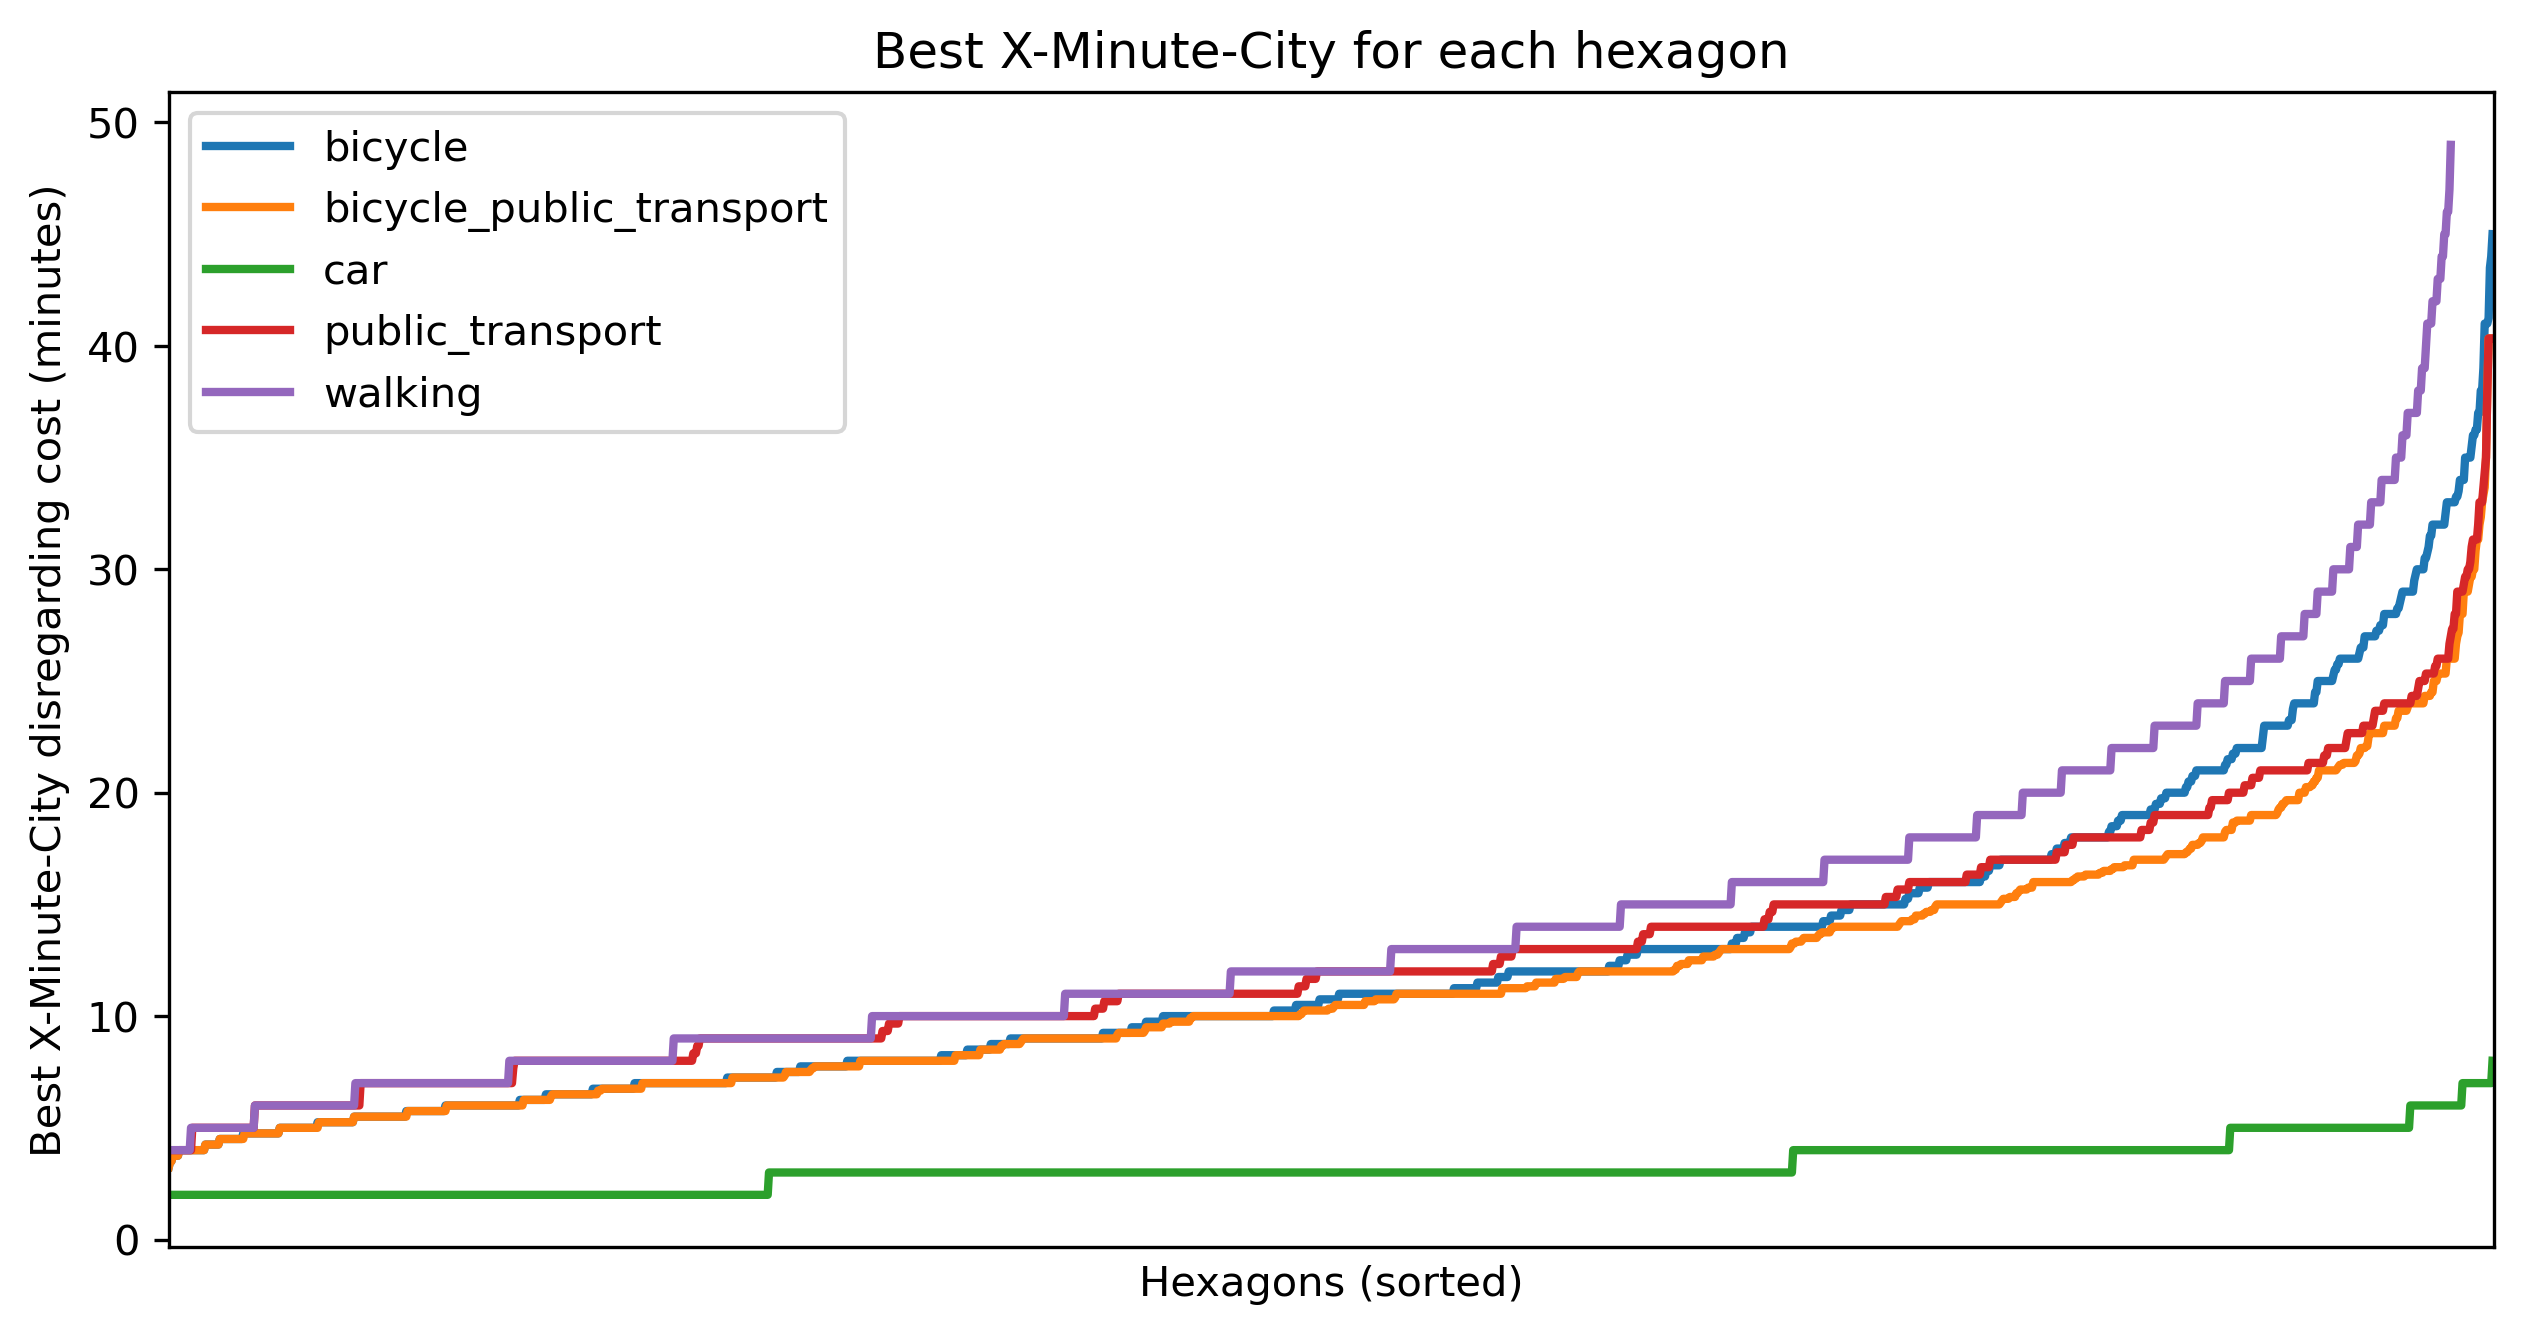
\includegraphics[width=0.65\textwidth]{Figures/results/minute_city_metric/best_x_minute_city}
  \end{center}
  \caption{Distribution of optimal x-minute city metric}
  \label{fig:optimal_x_minute_city_metric}
\end{figure}

As we can see initially (for the most accessible hexagons) public transport and walking are the same, but as we move to less accessible hexagons public transport becomes better.
In addition, the public transport scenario is worse than the pure bicycle sharing scenario, but is able to catch up to it and even overtake it as we move to less accessible hexagons.

The same pattern can be observed when comparing the bicycle sharing scenario to the combined scenario of bicycle sharing and public transport.
Initially, the combined scenario is the same as the bicycle sharing scenario, but as we move to less accessible hexagons the combined scenario becomes better.
Similarly, when comparing the bicycle sharing scenario to the combined scenario, we see that the combined scenario provides much better accessibility in the beginning but as we move to the least accessible hexagons both become the same.

Generally, we see that adding public transport is able to flatten the drastic increase of the optimal X-minute city metric at the end of the distribution.


Figure \ref{fig:optimal_map} shows the optimal X-minute city metric for each hexagon over all sustainable modes of travel, i.e. excluding the car scenario.

\begin{figure}
  \begin{center}
    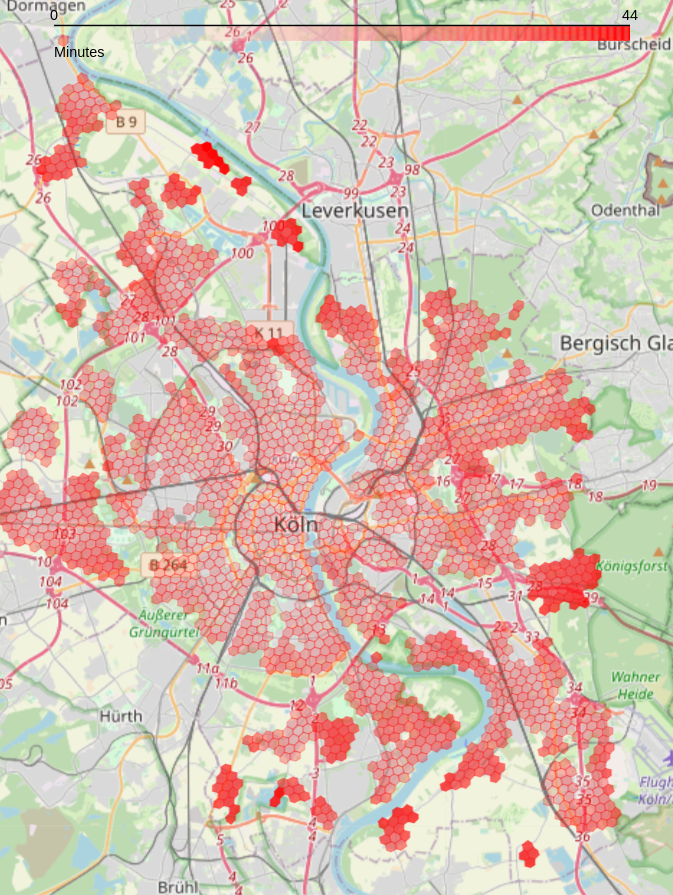
\includegraphics[width=0.45\textwidth]{Figures/results/minute_city_metric/optimal_map}
  \end{center}
  \caption{Map Of Optimal X-Minute City Metric}
  \label{fig:optimal_map}
\end{figure}

We can see that the least accessible hexagons require 44 minutes to reach all categories if only sustainable modes of travel are used.
The least accessible regions are in the suburban areas in the north and south of Cologne. 
Especially the region on the left side of the Rhine river next to Leverkusen, which is the district of Merkenenich, is very inaccessible.

Figure \ref{fig:optimal_map_per_scenario} shows multiple maps of the optimal X-minute city metric for each hexagon, one for bicycle sharing, one for public transport and one for walking.

\begin{figure}
     \centering
     \begin{subfigure}[b]{0.3\textwidth}
         \centering
         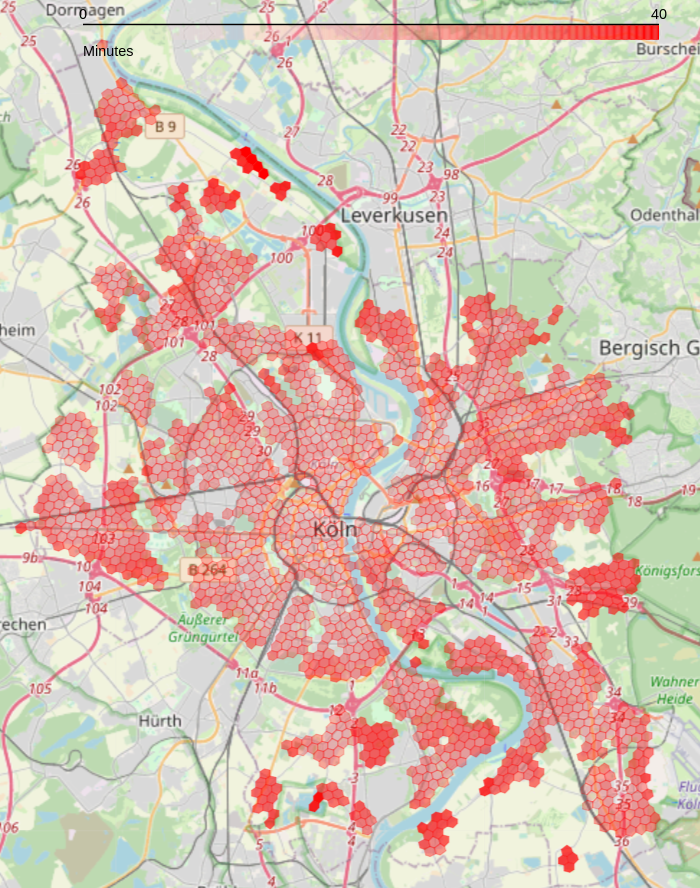
\includegraphics[width=\textwidth]{Figures/results/minute_city_metric/public_transport_optimal_map}
         \caption{Public Transport}
         \label{fig:public_transport_optimal_map}
     \end{subfigure}
     \hfill
     \begin{subfigure}[b]{0.3\textwidth}
         \centering
         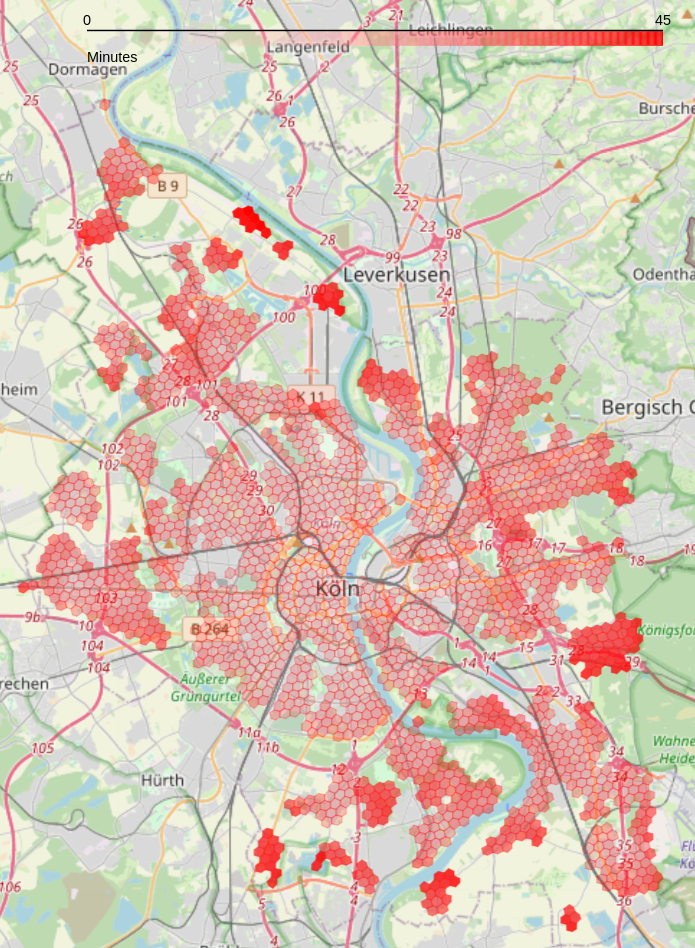
\includegraphics[width=\textwidth]{Figures/results/minute_city_metric/bicycle_optimal_map}
         \caption{Bicycle Sharing}
         \label{fig:bicycle_optimal_map}
     \end{subfigure}
     \hfill
     \begin{subfigure}[b]{0.3\textwidth}
         \centering
         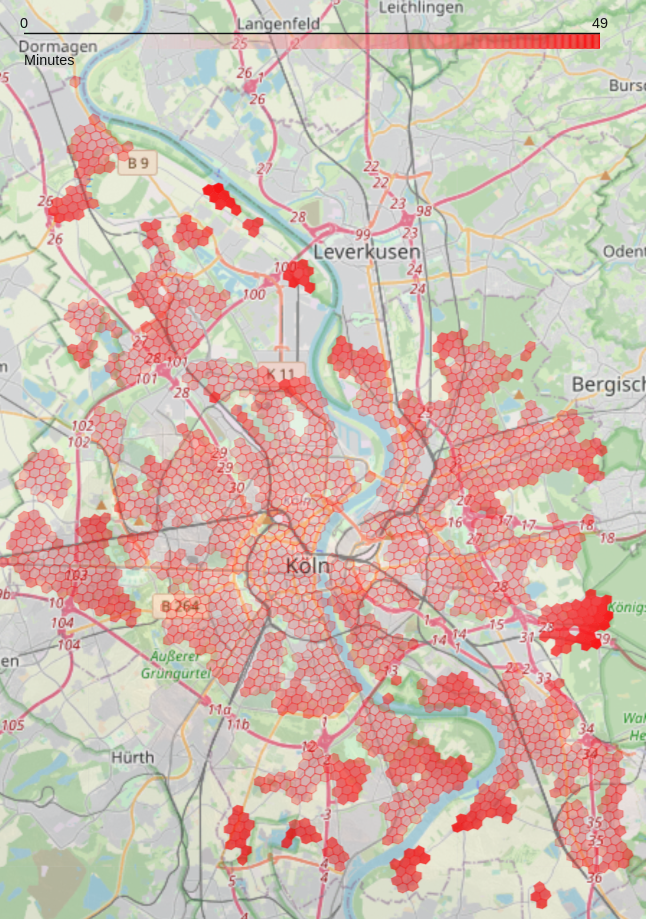
\includegraphics[width=\textwidth]{Figures/results/minute_city_metric/walking_optimal_map}
         \caption{Walking}
         \label{fig:walking_optimal_map}
     \end{subfigure}
        \caption{Map Of Optimal X-Minute City Metric Per Scenario}
        \label{fig:optimal_map_per_scenario}
\end{figure}

We see that the areas in and around the city center are more accessible by bicycle sharing than by public transport and walking.
At the east of the city, near the forest "Königsforst", we see the district of Rath/Neumar, with a low accessibility for all scenarios.
However, one can see that the region is more accessible by public transport than by bicycle sharing and walking.

\subsection{Cost Of 15-Minute City}
\label{subsec:cost_of_15_minute_city}

% table (mean, quantiles) of required cost
Table \ref{tab:required_cost} shows the mean, the 25\%, 50\% and 75\% quantiles and the max of the cost that are required to achieve the optimal value for the X-minute city.

\begin{table}
  \caption{Required cost for optimal over all hexagons}
  \label{tab:required_cost}
  \begin{center}
    \begin{tabular}{lrrrrr}
     & mean & 25\% & 50\% & 75\% & max \\
    scenario &  &  &  &  &  \\
    bicycle & 0.39 & 0.00 & 0.50 & 0.75 & 1.00 \\
    bicycle_public_transport & 0.87 & 0.00 & 0.75 & 1.30 & 3.95 \\
    car & 0.37 & 0.19 & 0.38 & 0.38 & 1.33 \\
    public_transport & 0.65 & 0.00 & 0.00 & 1.47 & 3.20 \\
    walking & 0.00 & 0.00 & 0.00 & 0.00 & 0.00 \\
    \end{tabular}
  \end{center}
\end{table}

We can immediately see that there is no cost for hexagons at the 25\% and 50\% quantile when using public transport.
Looking at the 75\% quantile and the maximum of the required cost for an optimal x-minute city metric for public transport, we see that the benefits we observed earlier come at a cost.

Similarly, comparing bicycle sharing to the combined scenario of bicycle sharing and public transport, we see that the maximum required cost is 4.20€ for the combined scenario, compared to 1.00€ for the bicycle sharing scenario.

We can make the same observation with more granularity when looking at the distribution of the required cost in Figure \ref{fig:maximum_required_cost_for_x_minute_city}.

\begin{figure}
  \begin{center}
    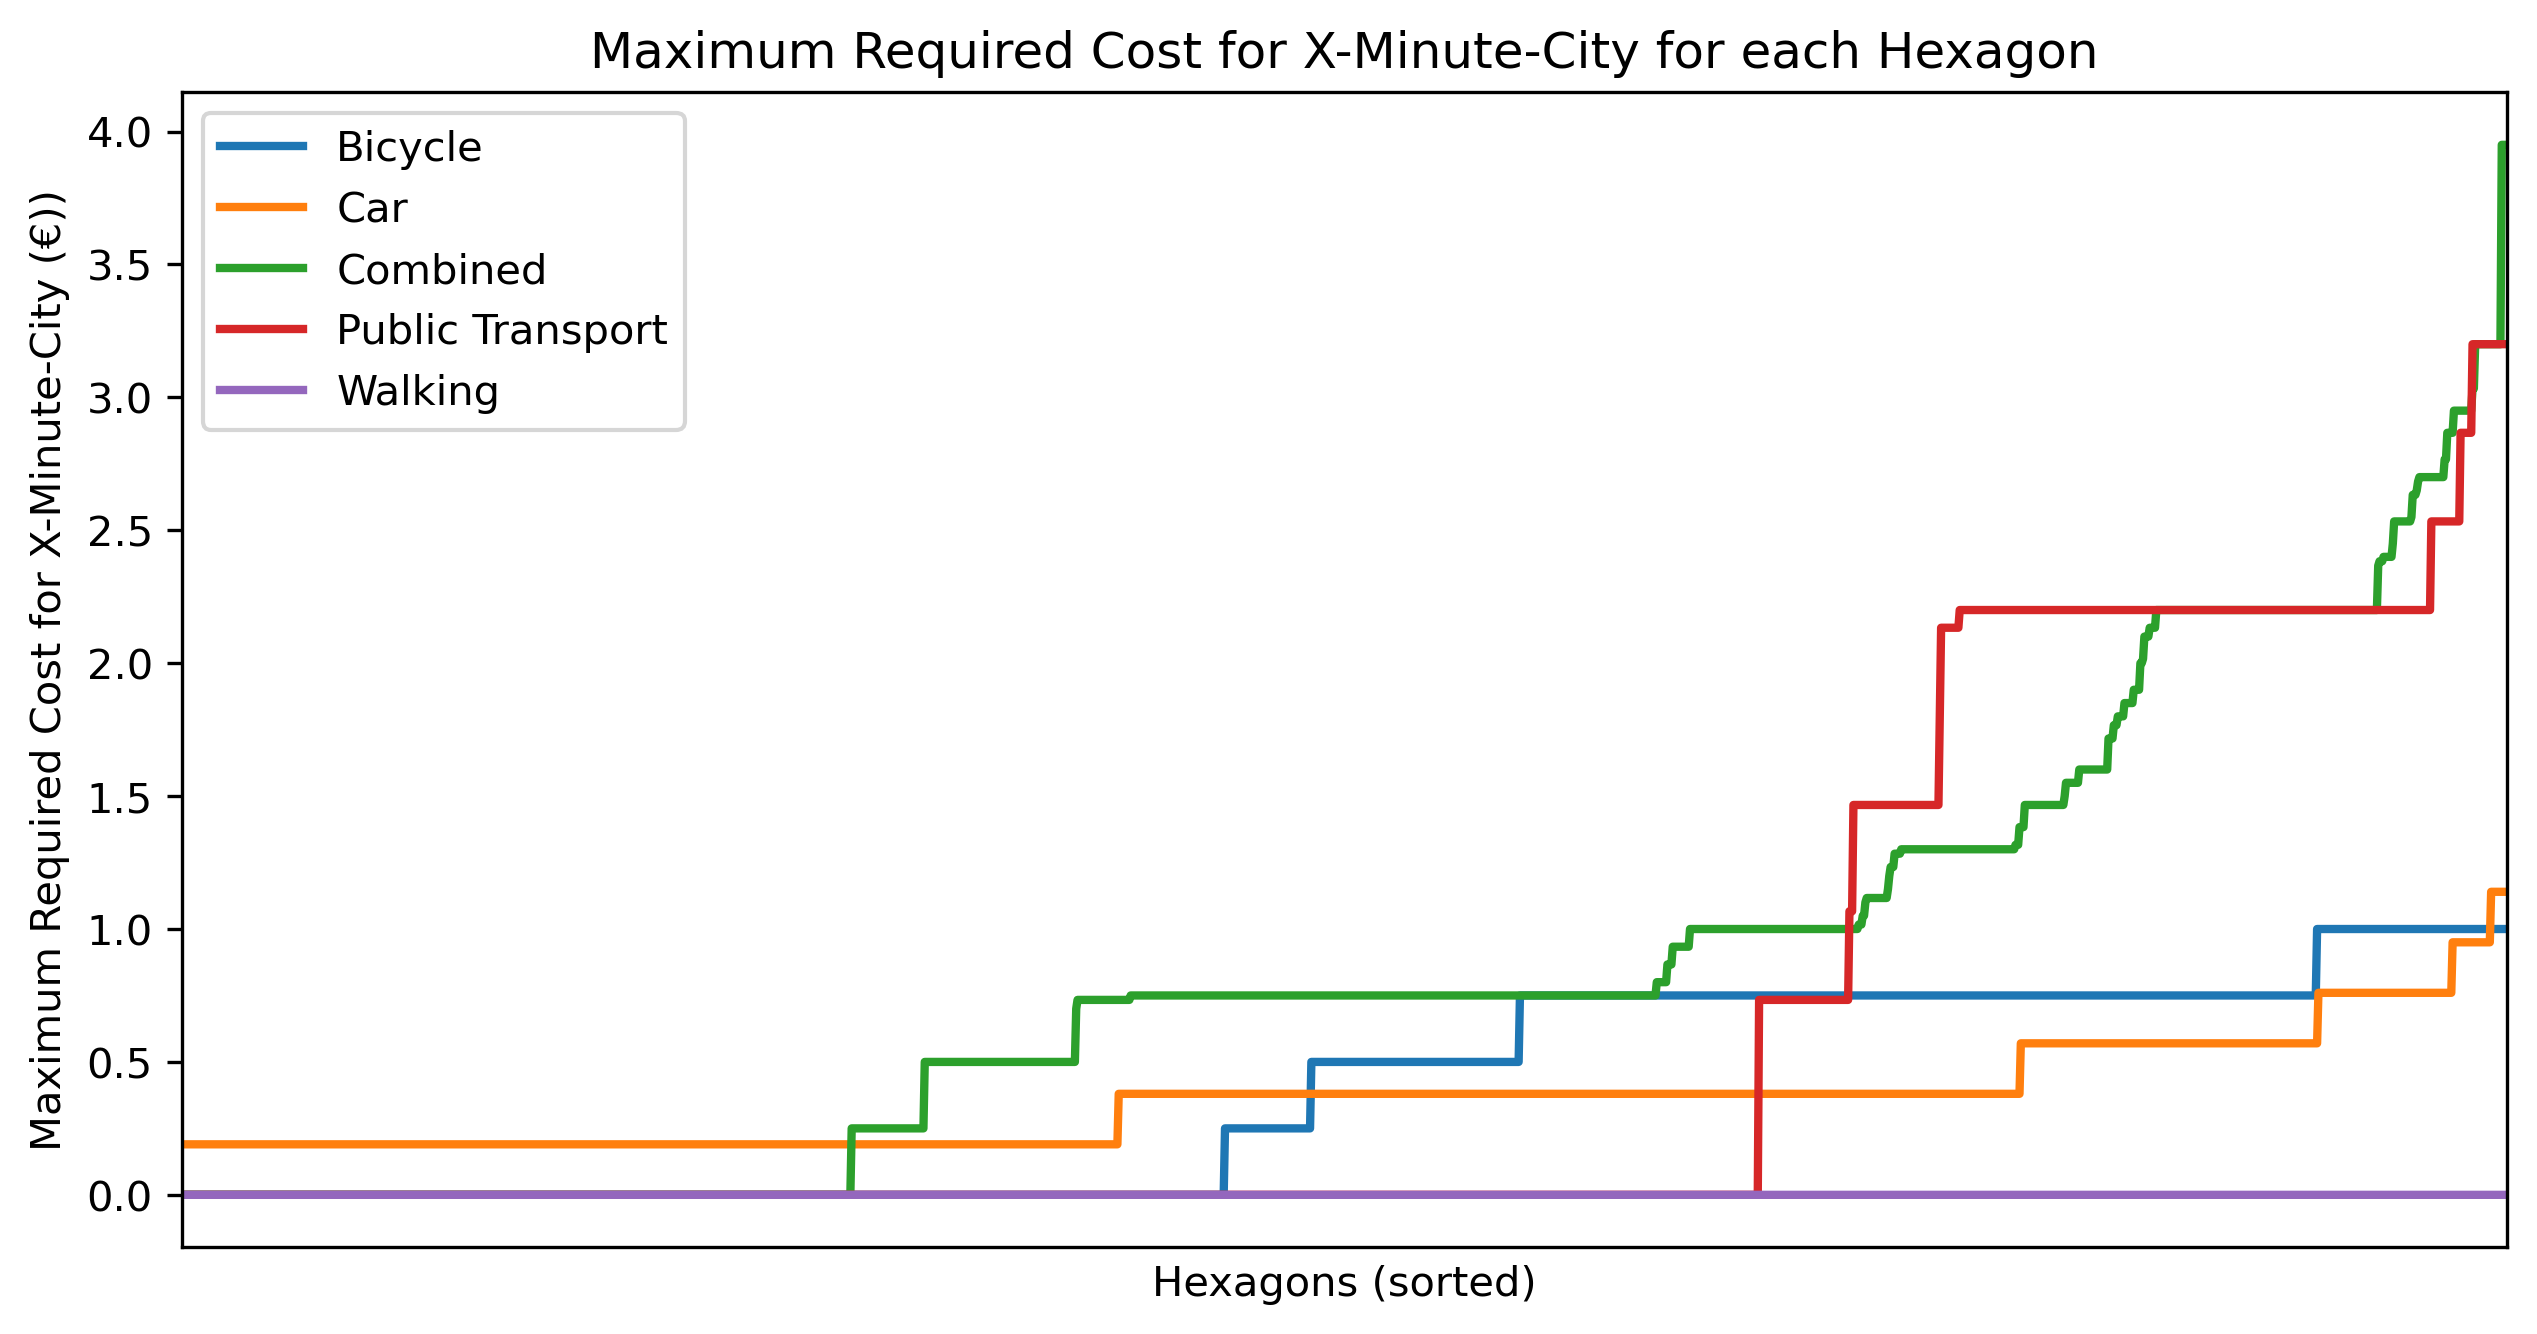
\includegraphics[width=0.65\textwidth]{Figures/results/cost/maximum_required_cost_for_x_minute_city}
  \end{center}
  \caption{Maximum required cost for optimal x-minute city metric}
  \label{fig:maximum_required_cost_for_x_minute_city}
\end{figure}

One interesting remark is that the maximum required cost for the bicycle sharing scenario is 1.00€, which implies that it is never necessary to use a bicycle more than 15 minutes to reach all categories.


Figure \ref{fig:cost_map_per_scenario} shows the cost required to reach the optimal X-minute city metric for each hexagon for public transport, bicycle sharing and the combined scenario of bicycle sharing and public transport.
Note that, we don't show the cost for the walking scenario, as it is always 0€.
In these figures, we see that sometimes the cost is zero.
As the portrayed scenarios all have costs associated with them, a cost of zero means that only walking is used.

\begin{figure}
     \centering
     \begin{subfigure}[b]{0.3\textwidth}
         \centering
         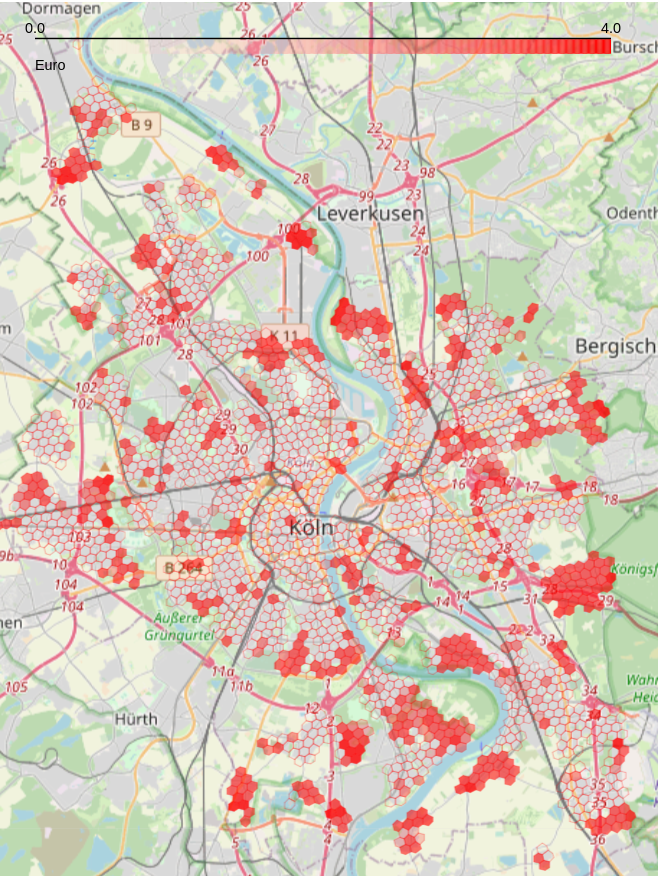
\includegraphics[width=\textwidth]{Figures/results/cost/public_transport_cost_map}
         \caption{Public Transport}
         \label{fig:public_transport_cost_map}
     \end{subfigure}
     \hfill
     \begin{subfigure}[b]{0.3\textwidth}
         \centering
         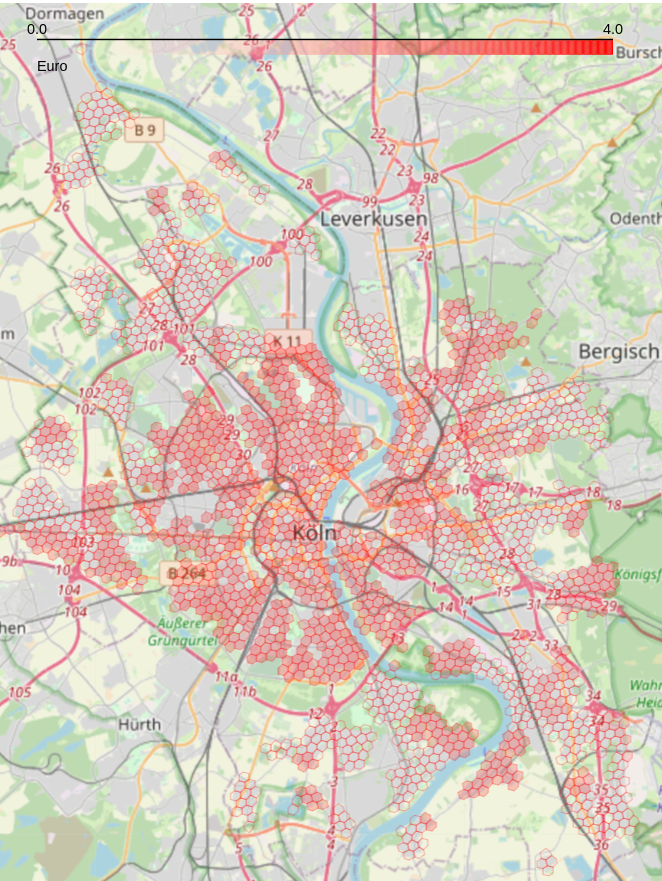
\includegraphics[width=\textwidth]{Figures/results/cost/bicycle_cost_map}
         \caption{Bicycle Sharing}
         \label{fig:bicycle_cost_map}
     \end{subfigure}
     \hfill
     \begin{subfigure}[b]{0.3\textwidth}
         \centering
         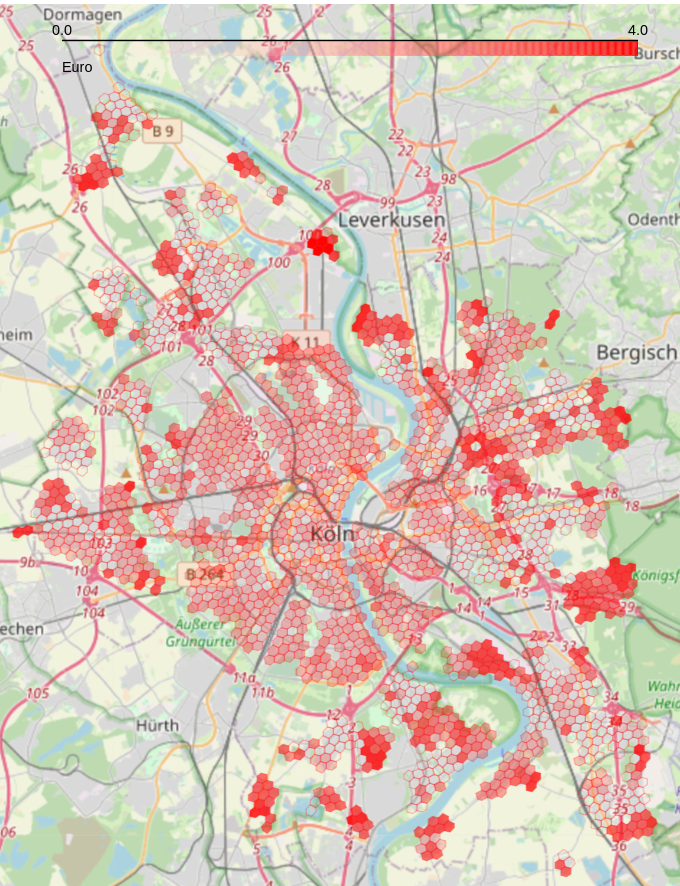
\includegraphics[width=\textwidth]{Figures/results/cost/bicycle_public_transport_cost_map}
         \caption{PT + Bicycle}
         \label{fig:bicycle_public_transport_cost_map}
     \end{subfigure}
       \caption{Map Of Required Cost For Optimal For Each Hexagon}
        \label{fig:cost_map_per_scenario}
\end{figure}


We see almost in all hexagons in and around the city center, where NextBike's flex zone is located, the cost for the bicycle sharing scenario is 1.00€.
This sometimes also extends outside the city center.
Other hexagons have a cost of 0.

The cost of public transport is more scattered around the whole region. We can mostly see single hexagons or small groups of hexagons that have a cost higher than 0.
Larger groups are only found outside the city center.

\subsection{Interaction Between Cost And 15-Minute City Metric}
\label{subsec:interaction_between_cost_and_15_minute_city_metric}

Next we are going to look at the interaction between the cost and the optimal X-minute city metric.
To do so we will investigate the mean Pareto front of the X-minute city metric and cost over all hexagons.
To understand this graph, we first take a look at the Pareto Front of a single hexagon.

Figure \ref{fig:example_pareto_front} shows an example Pareto Front for a single hexagon.
The x-axes show the cost and the y-axes show the X-minute city metric.
The curves show us what X-minute city is achievable for a given cost in specific scenario.

\begin{figure}
  \begin{center}
     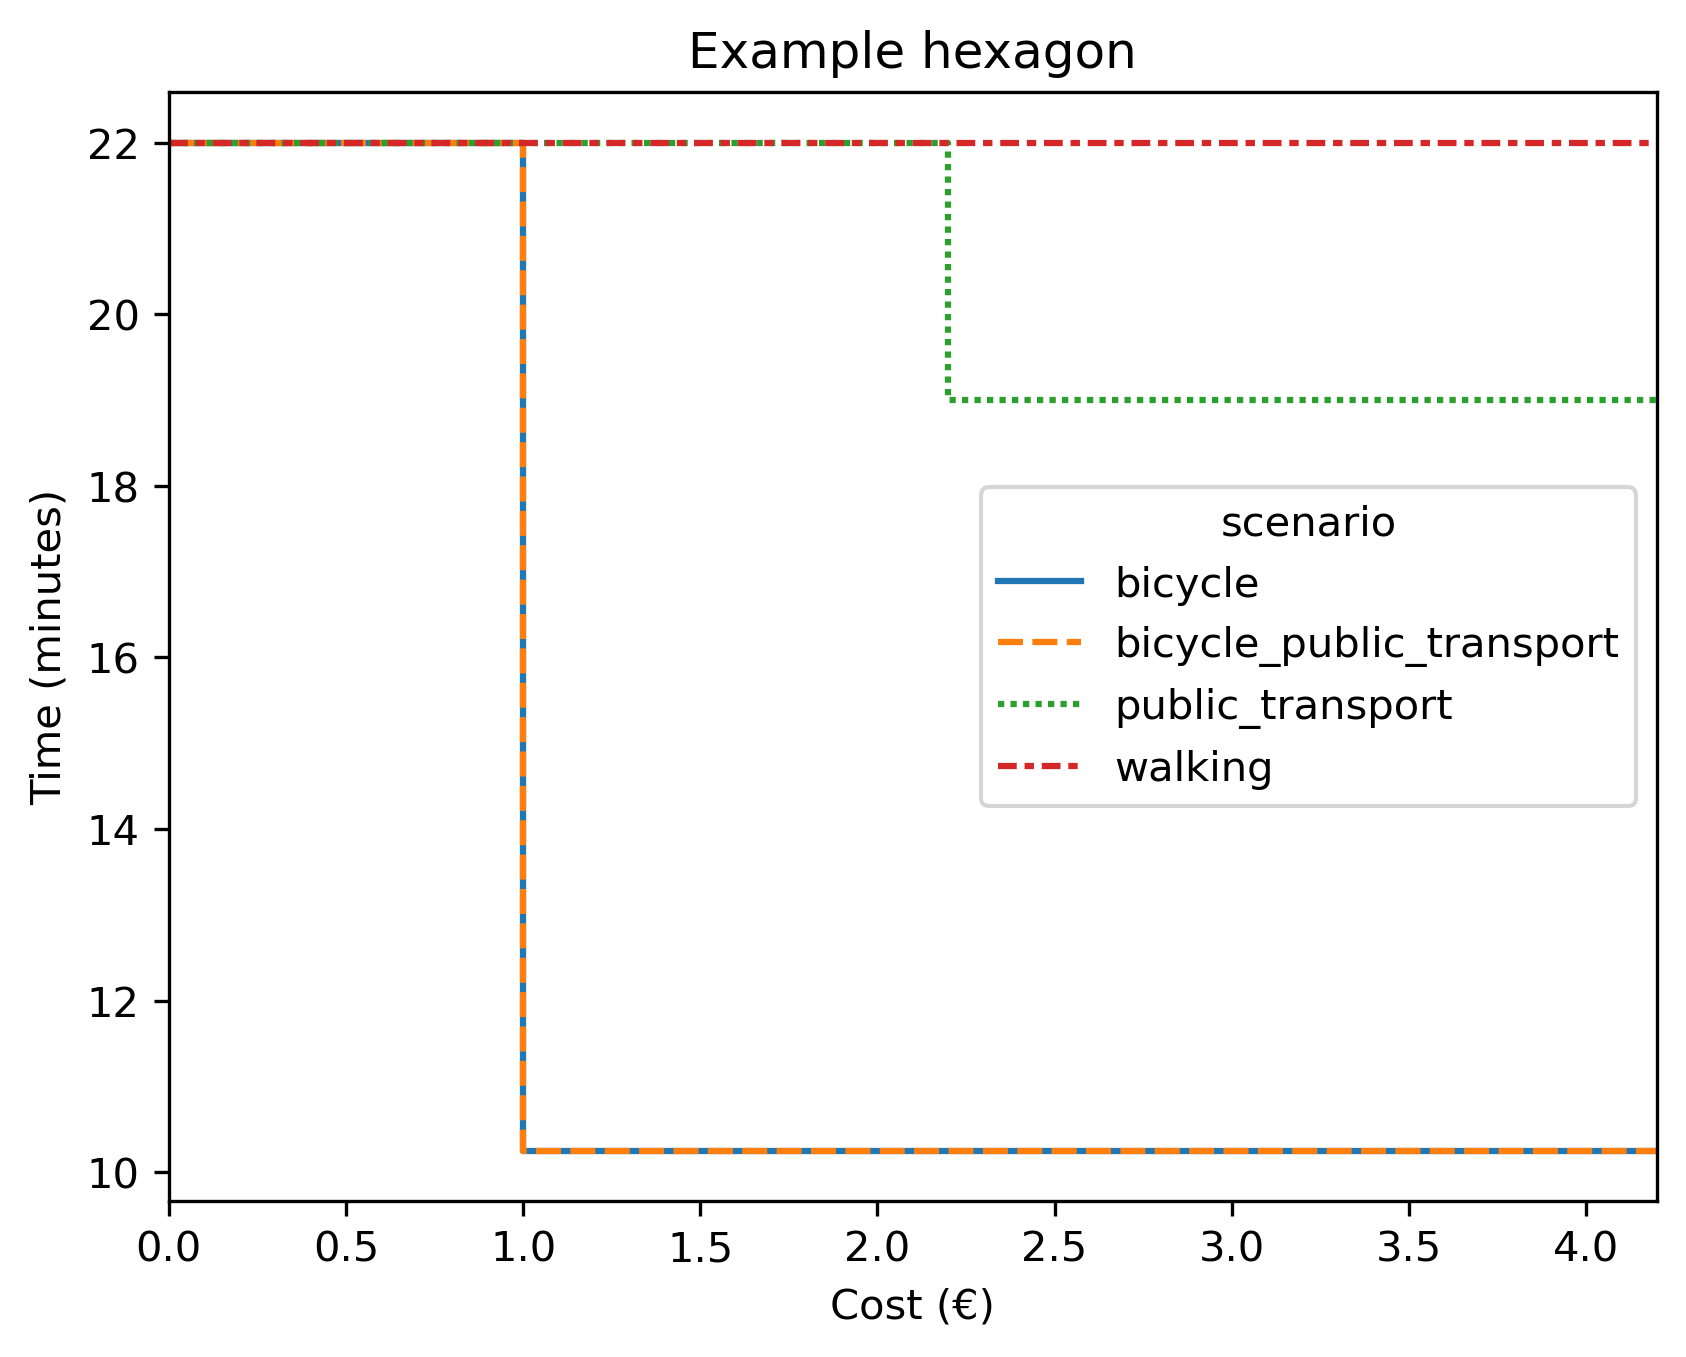
\includegraphics[width=0.5\textwidth]{Figures/results/metric_cost/example_profile}
  \end{center}
  \caption{Example Pareto Front}
  \label{fig:example_pareto_front}
\end{figure}

In our example, all modes begin with being able to reach all categories within 22 minutes for a cost of 0€.
Increasing, the cost only yields improves when reaching a cost of 1€, where the bicycle and combined scenario are able to reach all categories within approximately 10 minutes.
Further, increasing the price to 2.20€ yields an improvement for the public transport scenario, where it is now possible to reach all categories within approximately 19 minutes.
Further cost increases do not yield any improvements for any scenario.

We can also quantify the value of the improvements as seen in Table \ref{tab:differences_in_example_hexagon}.

\begin{table}
  \caption{Differences in example hexagon}
  \label{tab:differences_in_example_hexagon}
  \begin{center}
    \begin{tabular}{lrrrl}
    improvement & at cost & minute per euro & scenario \\
    11.75 & 1.00 & 11.75 & bicycle \\
    11.75 & 1.00 & 11.75 & bicycle_public_transport \\
    3.00 & 2.20 & 1.36 & public_transport \\
    \end{tabular}
  \end{center}
\end{table}

As we can see the bicycle scenarios' increase at a cost of 1€ is larger than the public transport scenario's increase and also has a higher value per euro.


% generalization
To generalize these findings over all hexagons we take the average over the X-minute city for each cost and scenario to generate an average Pareto front.
The resulting Pareto front can be seen in Figure \ref{fig:mean_time_per_cost}.

\begin{figure}
  \begin{center}
     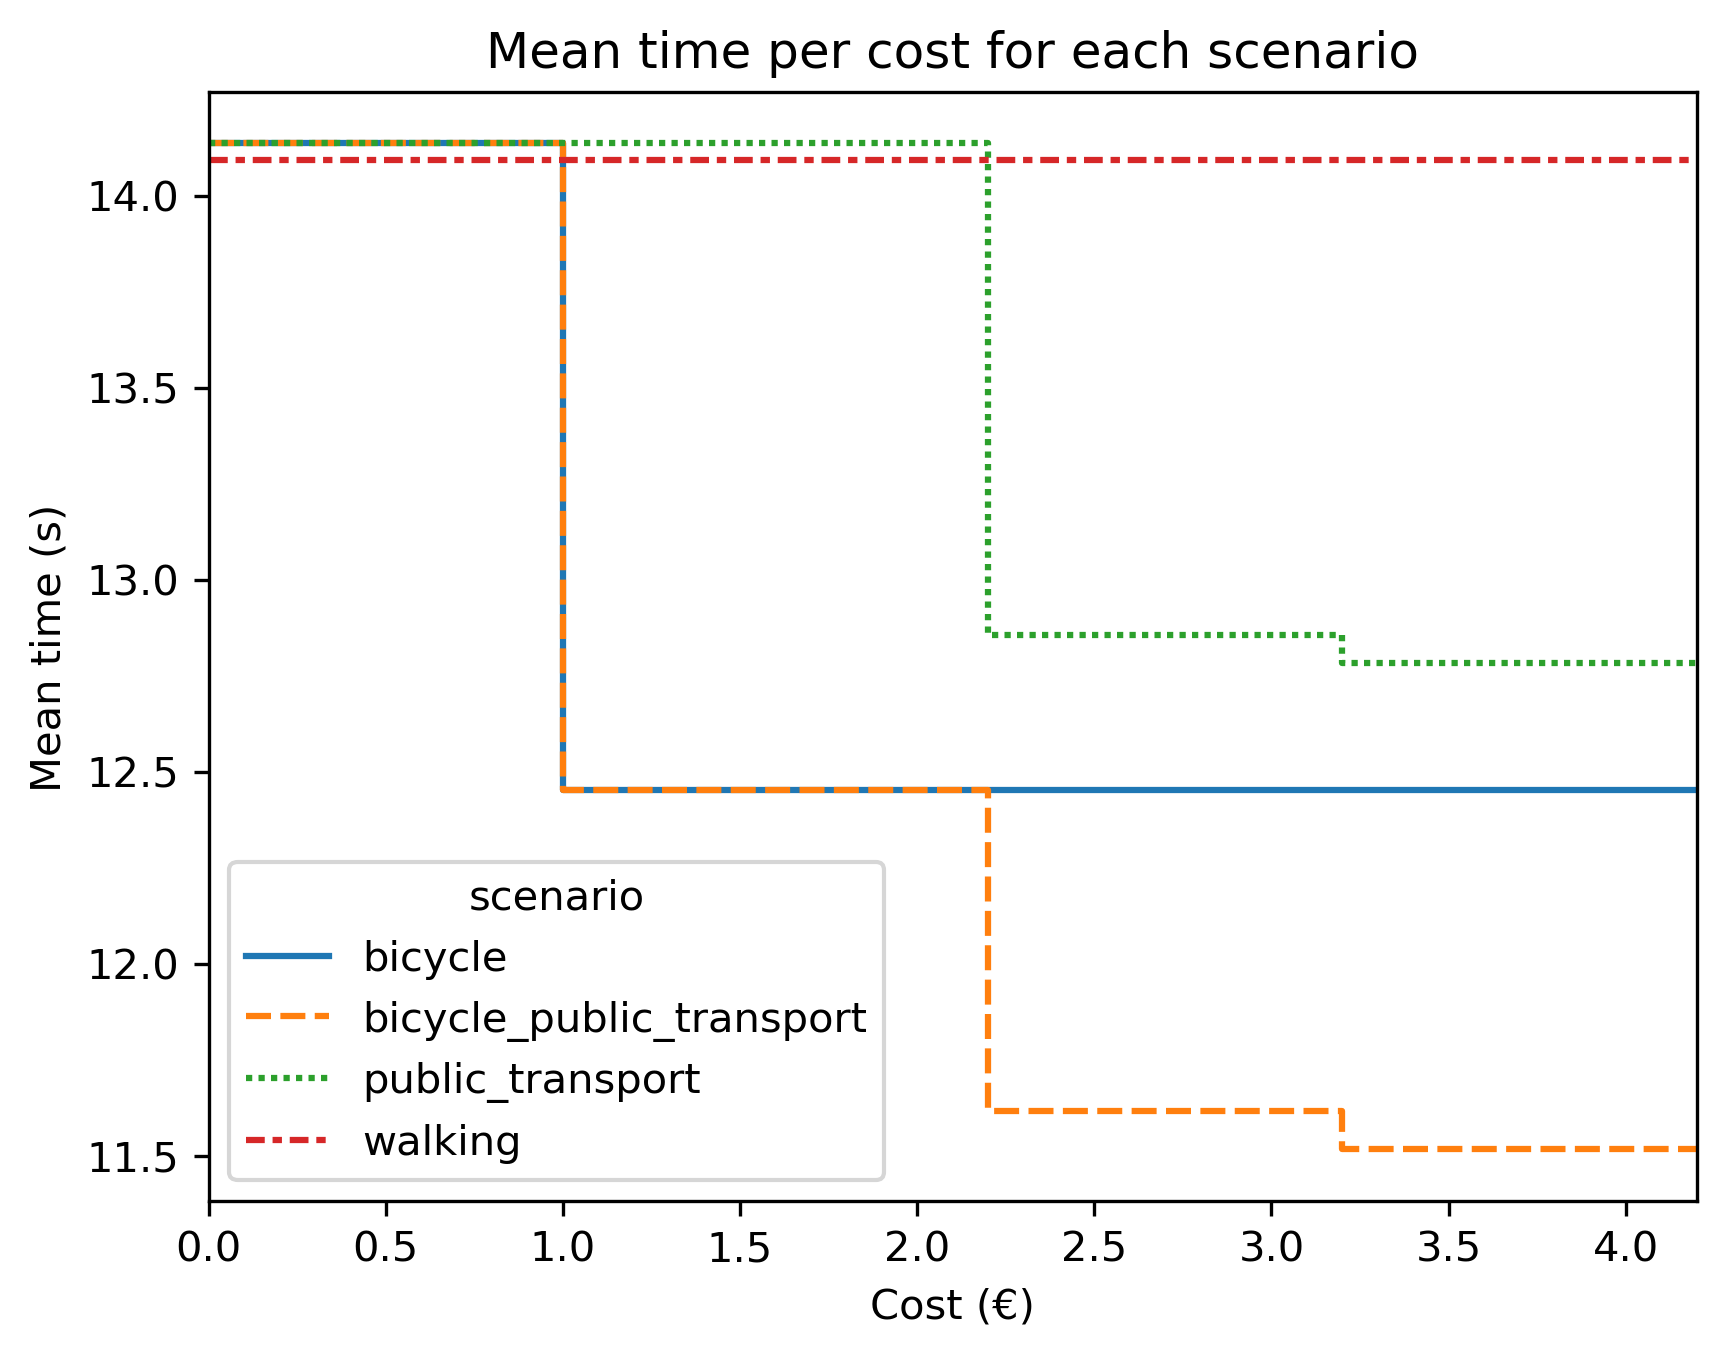
\includegraphics[width=0.5\textwidth]{Figures/results/metric_cost/mean_time_per_cost}
  \end{center}
  \caption{Mean time per cost for all scenarios}
  \label{fig:mean_time_per_cost}
\end{figure}

Similarly to the example of the single hexagon from before, we can see improvements for the bicycle scenario, as well as, the combined scenario at a cost of 1€ of about 1.5 minutes.
We can also see the improvements of public transport at a cost of 2.20€.
Unlike the example of the single hexagon, we can also see the improvement at a cost of 2.20€ for the combined scenario.
Lastly, there is also a slight improvement for the public transport scenario, as well as, the combined scenario at a cost of 3.20€.

To compare these improvements we can again look at the differences in Table \ref{tab:differences_in_mean_pareto_front}.
Note that we won't be analyzing the differences that occur in the combined scenario, as they may be skewed by prior improvements of other modes and are therefore hard to interpret.

\begin{table}
  \caption{Differences in mean Pareto front}
  \label{tab:differences_in_mean_pareto_front}
  \begin{center}
    \begin{tabular}{lrrrrl}
     & improvement & at cost & cost diff & minute per euro & scenario \\
     & 1.684 & 1.000 & 1.000 & 1.684 & bicycle \\
     & 1.282 & 2.200 & 2.200 & 0.583 & public transport \\
     & 0.074 & 3.200 & 1.000 & 0.074 & public transport \\
    \end{tabular}
  \end{center}
\end{table}

We see that the improvements of the bicycle scenarios at a cost of 1€ are the largest with an improvement of 1.68 minutes and also the most cost-effective with a value of 1.68 minutes per euro.
They are followed by the improvements of the public transport scenario at a cost of 2.20€ with an improvement of 1.28 minutes and a value of 0.58 minutes per euro.
The improvement at a cost of 3.20€ is very small and the least cost-effective.

Next, we are going to look at the quantiles of the aggregated Pareto front.
Figure \ref{fig:quantile_time_per_cost} shows the 25\%, 75\% and 90\% quantiles of the aggregated Pareto front.
The 25\% quantile gives us insights about the more accessible areas in the city.
Note that, because we aggregate all the values of the X-minute city metric for a single cost and scenario at a time, the 25\% quantile Pareto front does not necessarily reflect the same 25\% of hexagons for each cost.

\begin{figure}
     \centering
     \begin{subfigure}[b]{0.48\textwidth}
         \centering
         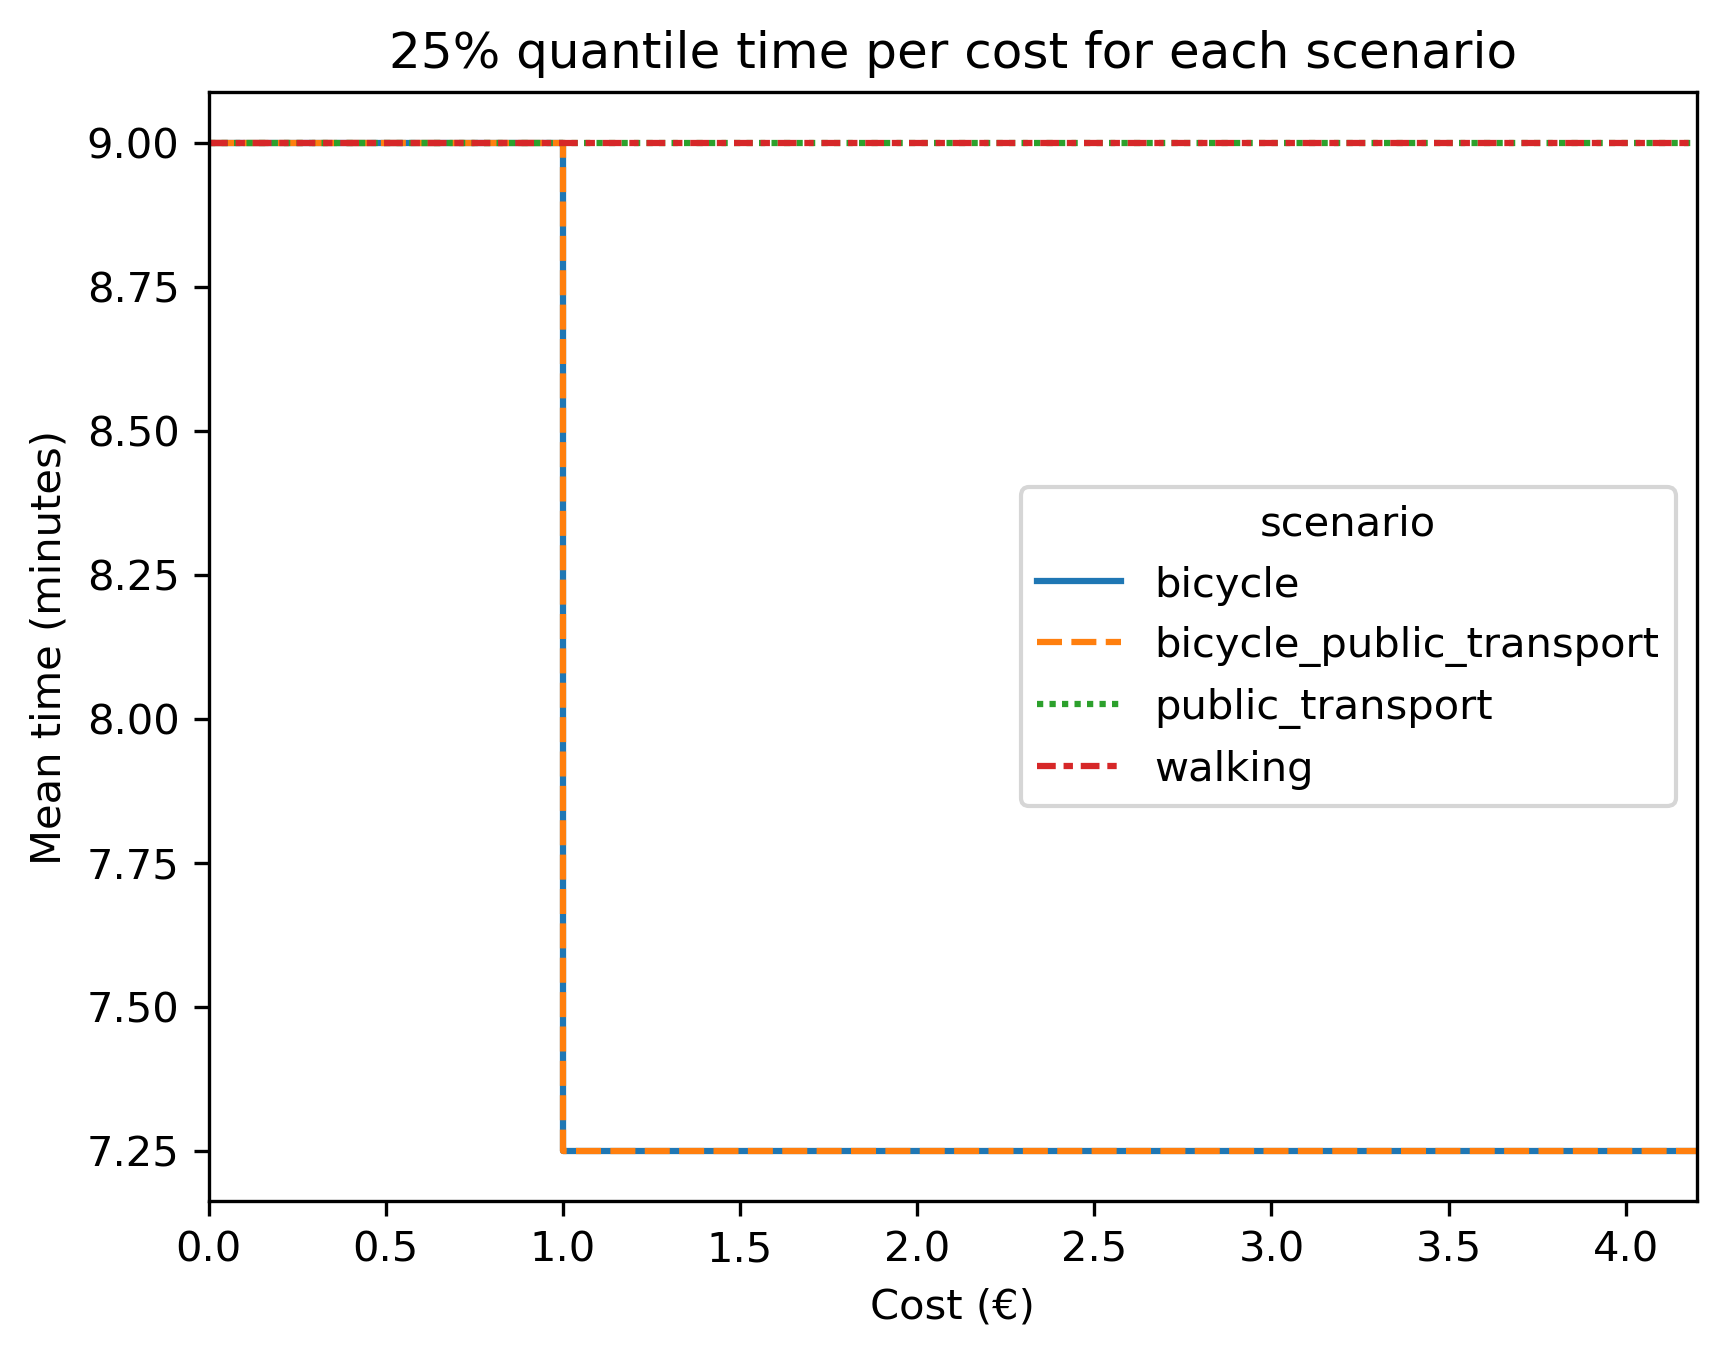
\includegraphics[width=\textwidth]{Figures/results/metric_cost/quantile_25_time_per_cost_for_each_scenario_without_car.png}
         \caption{25\% quantile time per cost for all scenarios}
         \label{fig:25_quantile_time_per_cost}
     \end{subfigure}
     \hfill
     \begin{subfigure}[b]{0.48\textwidth}
         \centering
         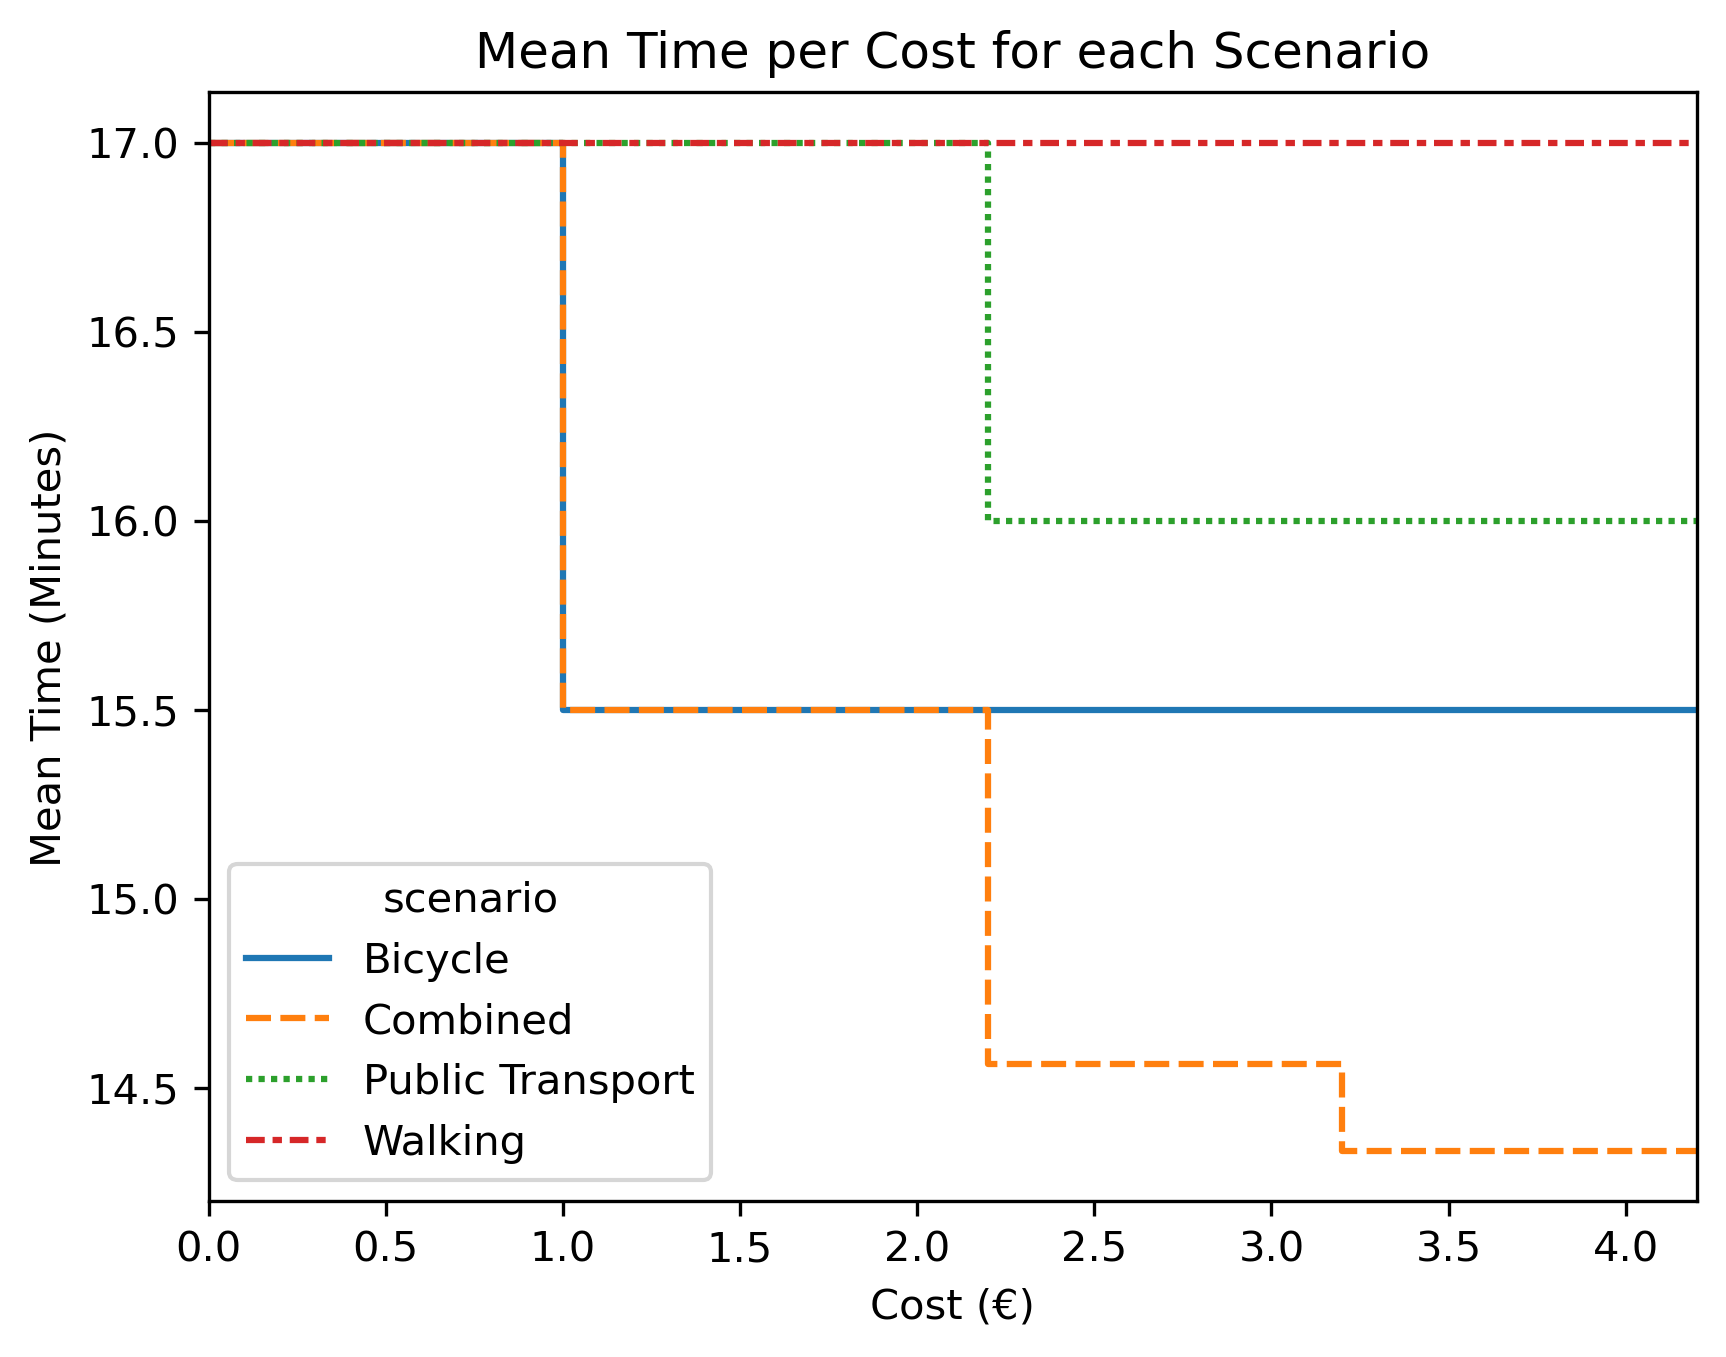
\includegraphics[width=\textwidth]{Figures/results/metric_cost/quantile_75_time_per_cost_for_each_scenario_without_car.png}
         \caption{75\% quantile time per cost for all scenarios}
         \label{fig:75_quantile_time_per_cost}
     \end{subfigure}
     \hfill
     \begin{subfigure}[b]{0.48\textwidth}
         \centering
         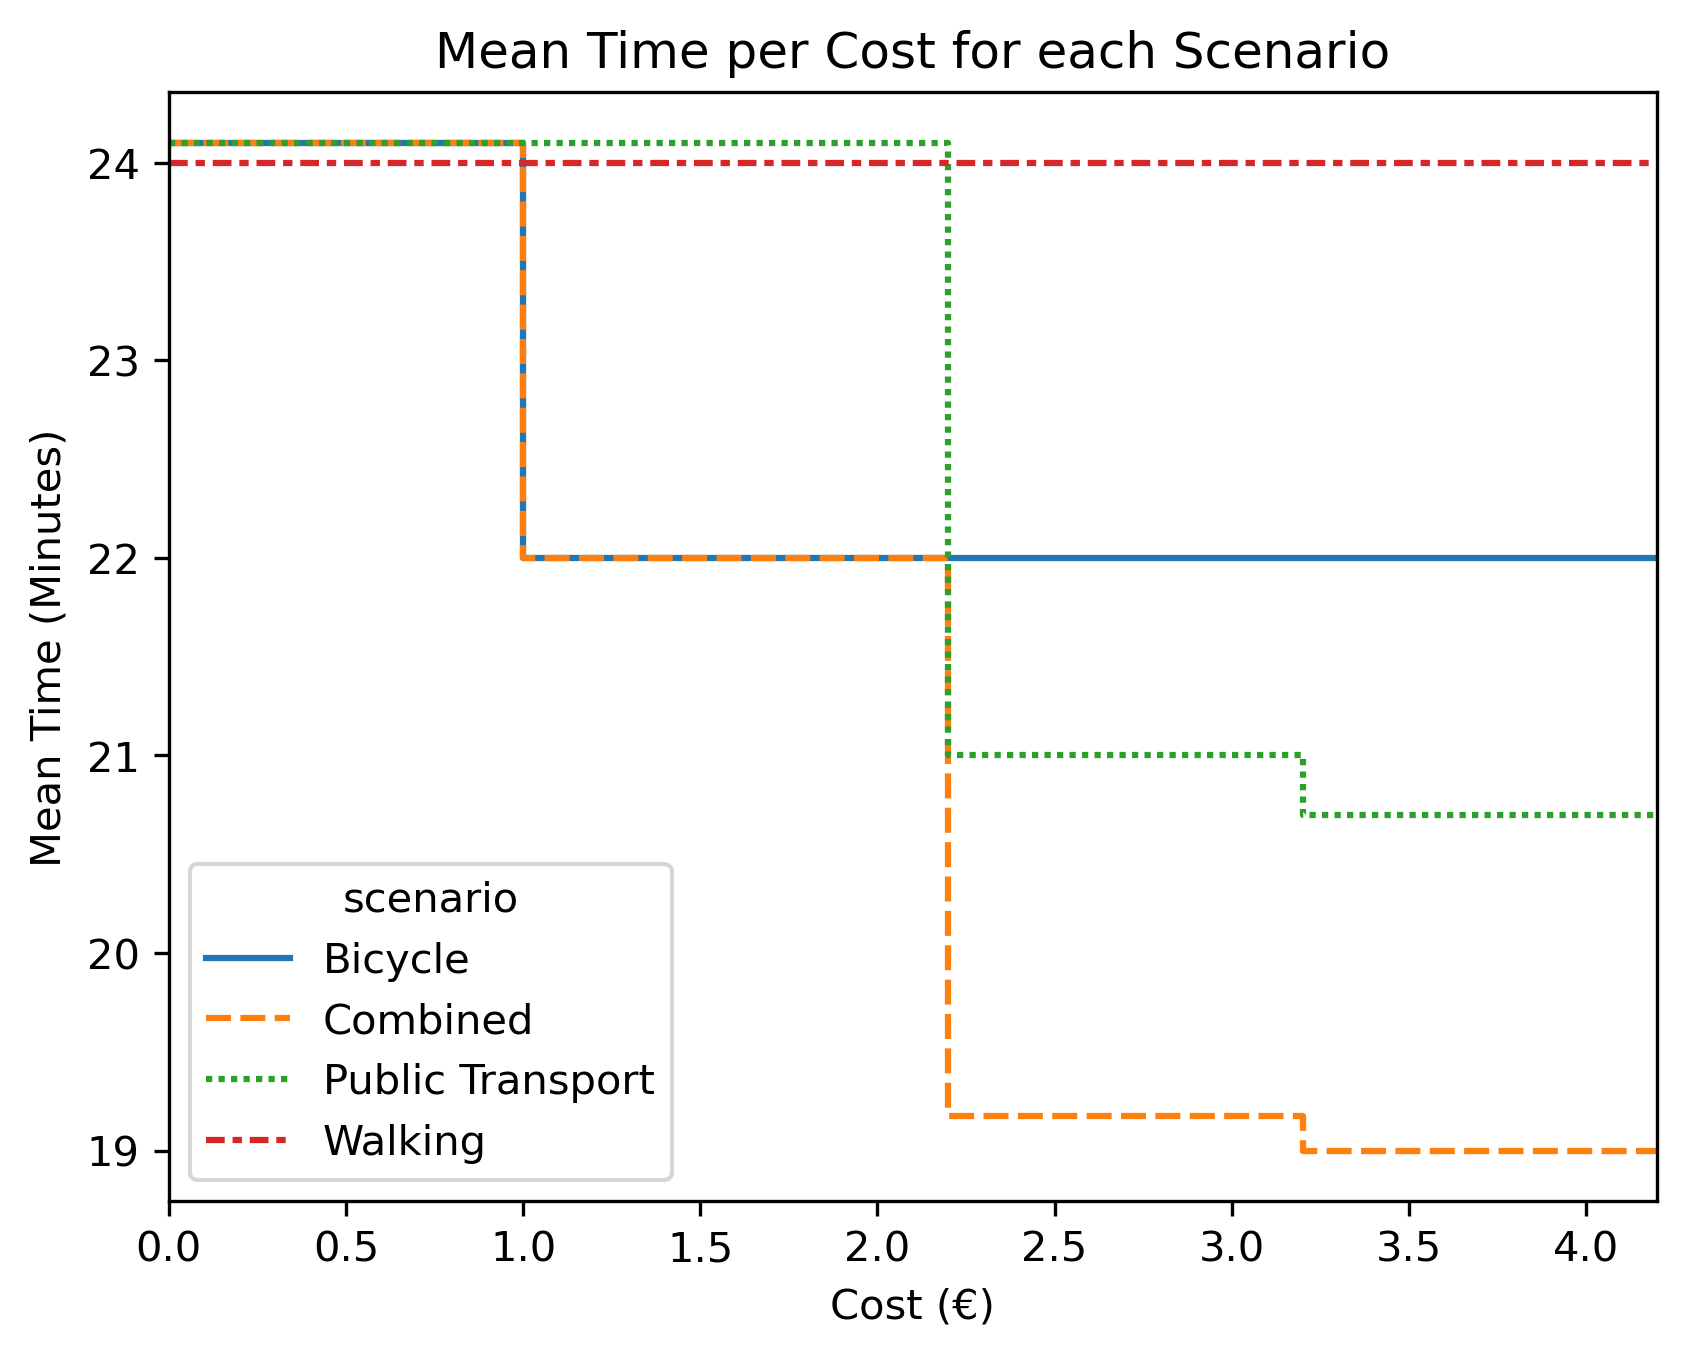
\includegraphics[width=\textwidth]{Figures/results/metric_cost/quantile_90_time_per_cost_for_each_scenario_without_car.png}
         \caption{90\% quantile time per cost for all scenarios}
         \label{fig:90_quantile_time_per_cost}
     \end{subfigure}
        \caption{Map Of Optimal X-Minute City Metric Per Scenario}
        \label{fig:quantile_time_per_cost}
\end{figure}

The 25\% quantile Pareto front shown in Figure \ref{fig:25_quantile_time_per_cost} only contains a single improvement at the cost of 1€ for bicycle related scenarios of 1.75 minutes with a cost-effectiveness of 1.75 minutes per euro.


The 75\% quantile Pareto front shown in Figure \ref{fig:75_quantile_time_per_cost} and Table \ref{tab:differences_in_75_quantile_pareto_front} also has a similar improvement of 1.5 minutes at the cost of 1€ for bicycle scenarios.
In addition to that, it also shows a smaller increase at 2.20€ for public transport scenarios of 1 minute and an even smaller increase at 3.20€ for bicycle sharing and public transport scenario.

\begin{table}
  \caption{Differences in 75\% quantile Pareto front}
  \label{tab:differences_in_75_quantile_pareto_front}
  \begin{center}
    \begin{tabular}{lrrrrl}
     improvement & at cost & cost diff & minute per euro & scenario \\
     1.500 & 1.000 & 1.000 & 1.500 & bicycle \\
     1.000 & 2.200 & 2.200 & 0.455 & public transport \\
    \end{tabular}
  \end{center}
\end{table}


The 90\% quantile Pareto Front shown in Figure \ref{fig:90_quantile_time_per_cost} and Table \ref{tab:differences_in_90_quantile_pareto_front} shows a similar pattern to the 75\% quantile Pareto front.
The major difference is that the increase at 2.20€ for public transport scenarios is larger than the increase at 1€ for bicycle scenarios.
More precisely, while bicycle sharing is more effective in decreasing the 15-minute city metric on average and also for the 75\% most accessible regions, public transport is more effective than bicycle sharing for the 10\% least accessible regions.
We should, however, note that even though the improvement in the public transport scenario is larger it is still less cost-effective than the improvement in the bicycle sharing scenario.


\begin{table}
  \caption{Differences in 90\% quantile Pareto front}
  \label{tab:differences_in_90_quantile_pareto_front}
  \begin{center}
    \begin{tabular}{lrrrrl}
     improvement & at cost & cost diff & minute per euro & scenario \\
     3.000 & 2.200 & 2.200 & 1.364 & public transport \\
     2.000 & 1.000 & 1.000 & 2.000 & bicycle \\
     0.033 & 3.200 & 1.000 & 0.033 & public transport \\
    \end{tabular}
  \end{center}
\end{table}


\subsection{Uncertainty/Subscenarios}
\label{subsec:uncertainty_subscenarios}

As some of our input data is subject to uncertainties, we need to investigate the effects of this uncertainty in order to establish the robustness of our results.

First, we are going to look at the average standard deviation of the optimal value for the X-minute city metric in Table \ref{tab:average_standard_deviation_of_optimal_value_for_x_minute_city_metric}, effectively showing the standard deviation of the values in Table \ref{tab:optimal_x_minute_city_metric}.
Note, that we display the average standard deviations of the bicycle, public transport and combined scenario as those are the only ones with uncertainty.

\begin{table}
  \caption{Average standard deviation of optimal value for X-minute city metric}
  \label{tab:average_standard_deviation_of_optimal_value_for_x_minute_city_metric}
  \begin{center}
    \begin{tabular}{lrrrrrrr}
     & mean & min & 25\% & 50\% & 75\% & max & CV \\
    scenario &  &  &  &  &  &  &  \\
    bicycle & 1.16 & 0.00 & 0.00 & 0.50 & 1.73 & 13.15 & 0.093403 \\
    bicycle_public_transport & 0.94 & 0.00 & 0.00 & 0.74 & 1.48 & 6.73 & 0.082027 \\
    public_transport & 0.27 & 0.00 & 0.00 & 0.00 & 0.00 & 8.66 & 0.021151 \\
    \end{tabular}
  \end{center}
\end{table}


We see that the mean average standard deviation for bicycle scenarios is around a minute, while it is 0.27 for the public transport scenario.
We can also see that for the bicycle related scenarios the uncertainty does not affect the 25\% most accessible hexagons, while for public transport the 75\% most accessible hexagons are not affected.
In addition, we see that outliers exist with more than 10 minutes of deviation for the pure bicycle scenario and more than 5 minutes of deviation for the public transport related scenarios.
Relating the standard deviation to the mean we also calculated the Coefficient of Variation (CV) to the table, which is calculated as follows:
$$ CV = \frac{\sigma}{\mu} $$
where $\mu$ is the mean and $\sigma$ is the standard deviation.
We see that it is approximately 9\% for the bicycle related scenarios and 2\% for the public transport scenario.

To further investigate the effects of uncertainty on a more granular level, we plot the distribution of the optimal X-minute city for each hexagon in Figure \ref{fig:best_and_worst_case_of_optimal_time_for_each_hexagon}.
These plots are essentially the upper and lower bounds of the graph as seen in Figure \ref{fig:optimal_x_minute_city_metric}.
In addition, we've added a line at the 15-minute mark, to better relate the results in context of the 15-minute city.


\begin{figure}
  \begin{center}
    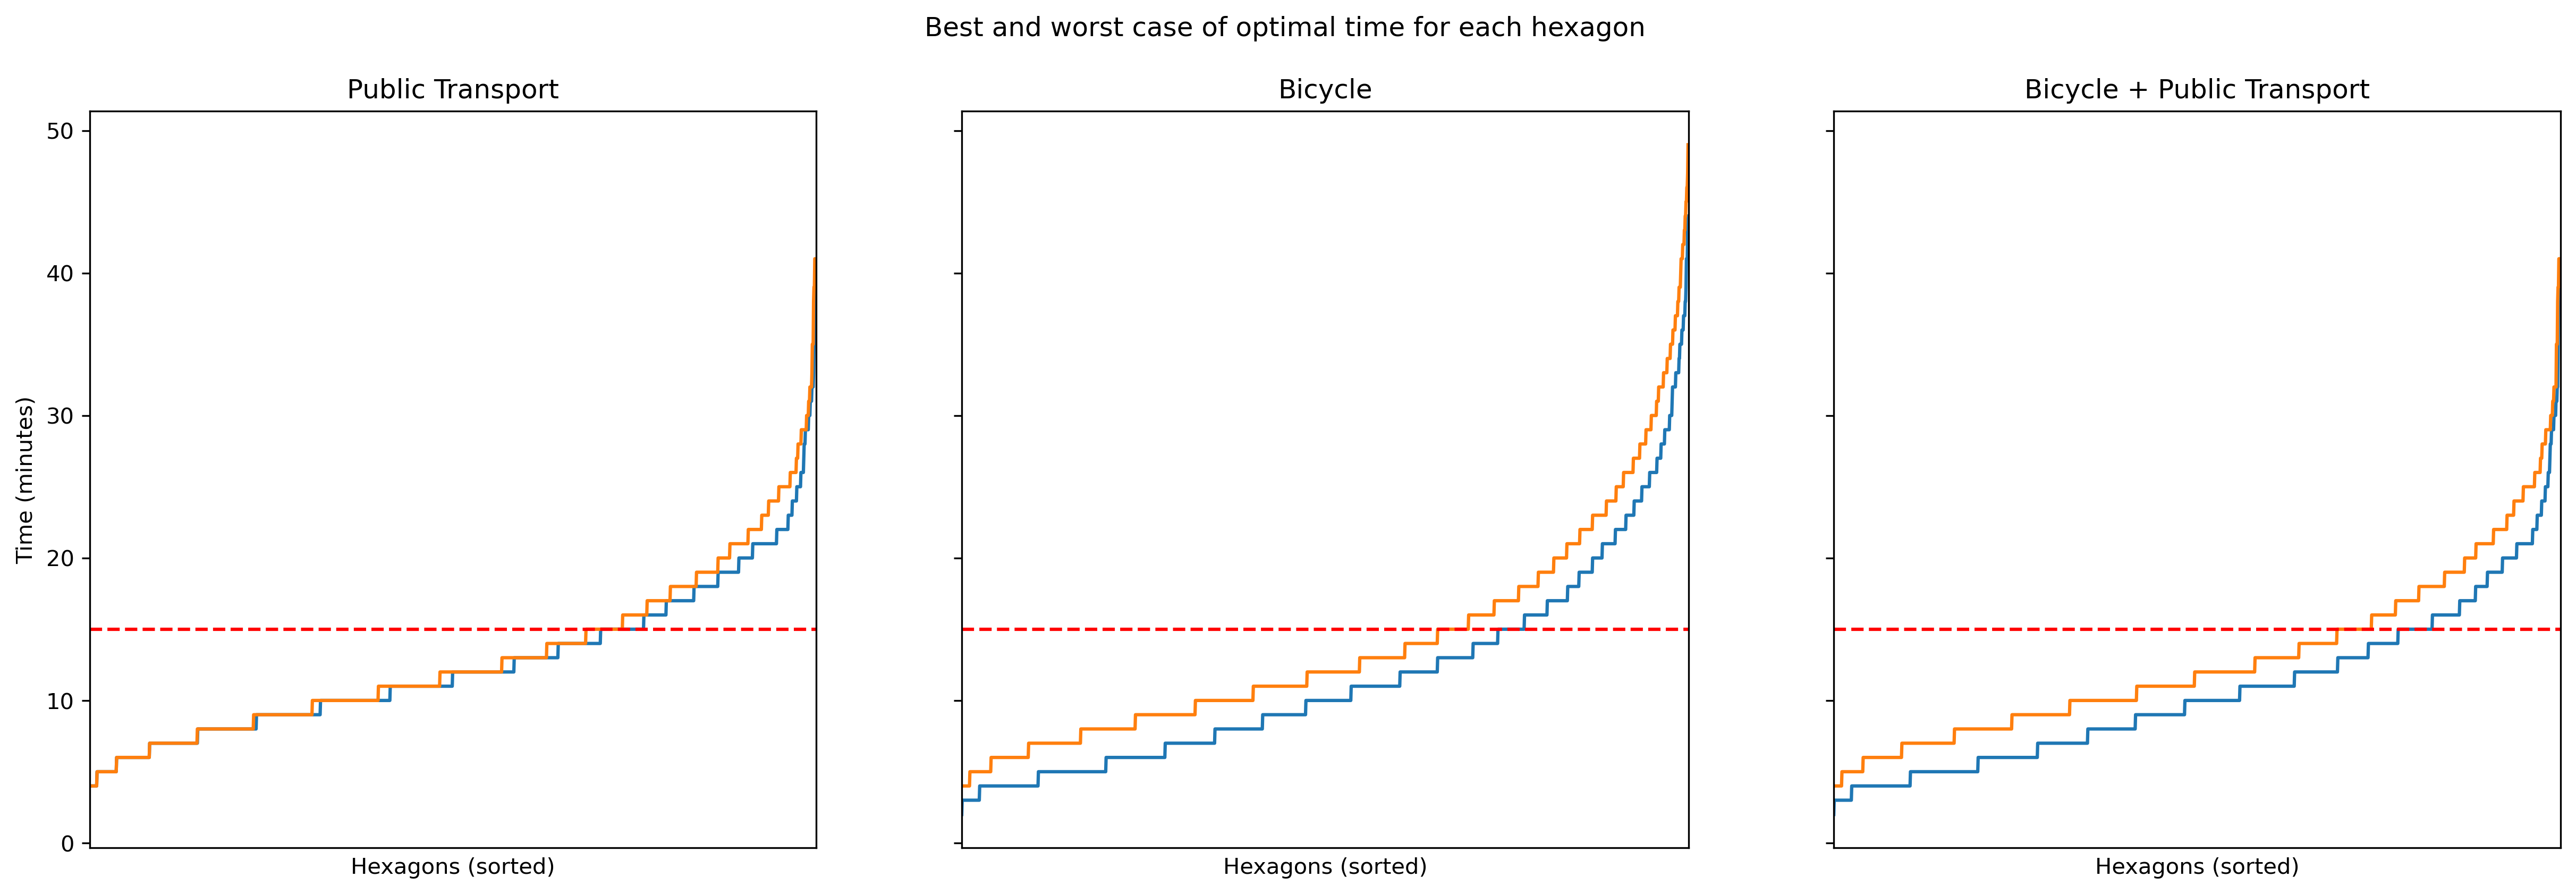
\includegraphics[width=0.95\textwidth]{Figures/results/uncertainty/optimal_best_worst_case}
  \end{center}
  \caption{Best and worst case of optimal time for each hexagon}
  \label{fig:best_and_worst_case_of_optimal_time_for_each_hexagon}
\end{figure}

First, we see that the variation for bicycles is spread out over almost all hexagons, in comparison to public transport where the variation only really begins to happen after the 15-minute mark.
For the combined scenario, we see the expected: the variances of the public transport scenario and the bicycle scenario add up.

\subsection{Impact Of Sustainable Modes On 15-Minute Metric}
\label{subsec:impact_of_sustainable_modes_on_15_minute_metric}

To analyze the impact of sustainable modes of travel on the 15-minute city metric, we first uncover the problematic areas, in which the X-minute city metric is above 15 minutes for the walking mode.
We then analyze how the sustainable modes of travel can help to reduce the X-minute city metric in those areas below 15 minutes.

In total, we find 552 hexagons, which have a walking time of more than 15 minutes to reach all categories, which is 30.98\% of all hexagons.

\begin{table}[h]
  \centering
  \begin{tabular}{|l|l|}
    \hline
    \textbf{Category}                                          & \textbf{Data}                \\ \hline
    Only bicycle below 15 mins                                 & 72 (13.04\%)                 \\ \hline
    Only public transport below 15 mins                        & 59 (10.69\%)                 \\ \hline
    Both bicycle and public transport below 15 mins            & 41 (7.43\%)                  \\ \hline
    Combined mode below 15 mins                                & 10 (1.81\%)                  \\ \hline
    Not reachable by sustainable modes below 15 mins           & 370 (67.03\%)                \\ \hline
  \end{tabular}
  \caption{Impact of Sustainable Modes on Reducing Walking Time Above 15 Minutes}
  \label{table:hexagons_with_walking_time_above_15_minutes}
\end{table}
% TODO make this a pie chart?

Table \ref{table:hexagons_with_walking_time_above_15_minutes} presents the distribution of hexagons with a walking time above 15 minutes and the effect of sustainable transportation modes on these times. 
A significant portion of these areas, amounting to 67.03\%, cannot be reached within 15 minutes using sustainable modes with the current state of infrastructure. 
Conversely, the data indicates that for 13.04\% of these hexagons, bicycles alone can reduce travel time to under 15 minutes, while public transport alone can achieve this for 10.69\% of the hexagons. 
7.43\% of hexagons are reachable with either one of bicycles or public transport, while an additional 1.81\% of hexagons are accessible within this time frame when combining  modes. 


Next we visualize these problematic areas spatially.
Figure \ref{fig:problematic_hexagons} shows hexagons where all necessities are reachable within a 15-minute walk in green, hexagons where all necesseities are reachable within 15-minutes via some form of sustainable travel in yellow, and hexagons where all necessities are not reachable within 15 minutes in red.

\begin{figure}
  \begin{center}
    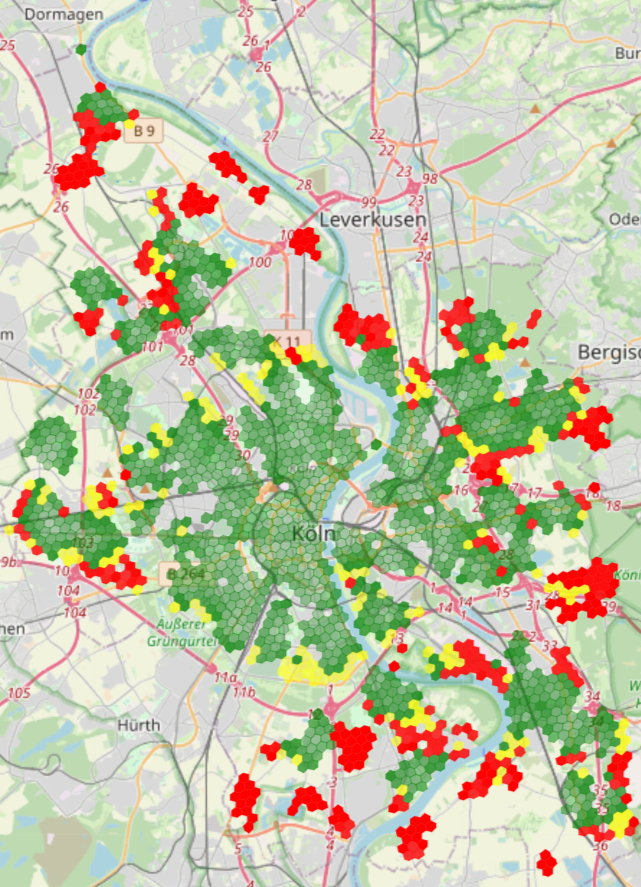
\includegraphics[width=0.50\textwidth]{Figures/results/problematic_hexagons/problematic_hexagons}
  \end{center}
  \caption{Unfixable, fixable and unproblematic hexagons on a map}
  \label{fig:problematic_hexagons}
\end{figure}

We see that in the center of Cologne, almost all hexagons qualify as 15-minute city hexagons. 
At the border of the city, we clearly see a yellow ring.

Most hexagons that never qualify as 15-minute city hexagons are located in suburban area, often in larger groups.

Next we take a look at the hexagons previously colored yellow, namely those where bicycles and public transport or a combination of both can decrease the 15-minute city metric below 15 minutes.
Figure \ref{fig:fixable_hexagons} shows hexagons that are 15-minute city hexagons through public transport in yellow, hexagons that are 15-minute city hexagons through bicycle sharing in orange and hexagons that are 15-minute city hexagons through either in green.

\begin{figure}
  \begin{center}
    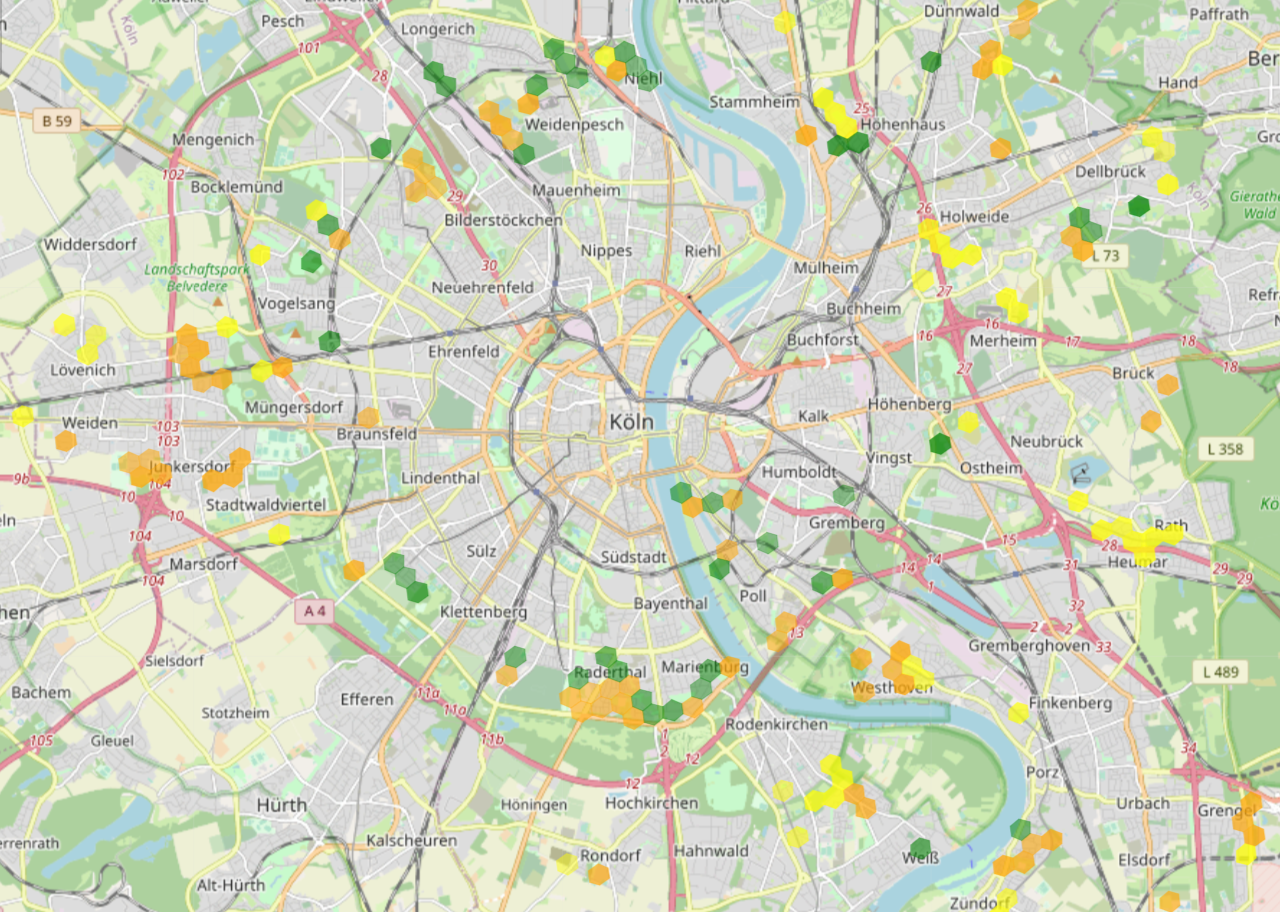
\includegraphics[width=0.50\textwidth]{Figures/results/problematic_hexagons/fixable_hexagons}
  \end{center}
  \caption{Fixable hexagons by mode}
  \label{fig:fixable_hexagons}
\end{figure}

We see a slight tendency that hexagons that become 15-minute city hexagons only through bicycle sharing (orange) are closer to the city center than those that become 15-minute city hexagons only through public transport. 

The outer clusters of fixable hexagons correlates directly with the locations of bicycles and public transport stops.
Figure \ref{fig:fixable_hexagons_examples} shows four zoomed in excerpts from Figure \ref{fig:fixable_hexagons}.

\begin{figure}
     \centering
     \begin{subfigure}[b]{0.45\textwidth}
         \centering
         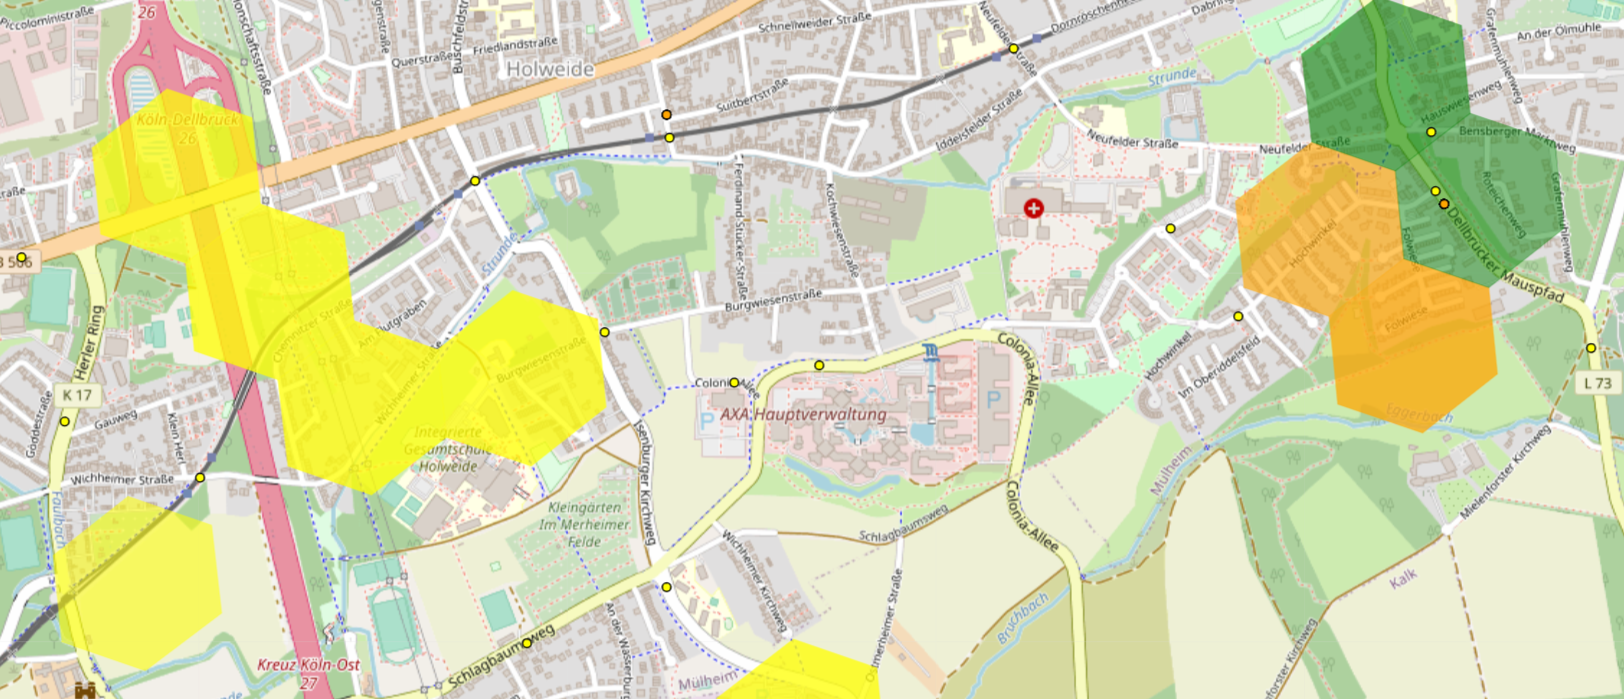
\includegraphics[width=\textwidth]{Figures/results/problematic_hexagons/example_1.png}
     \end{subfigure}
     \hfill
     \begin{subfigure}[b]{0.45\textwidth}
         \centering
         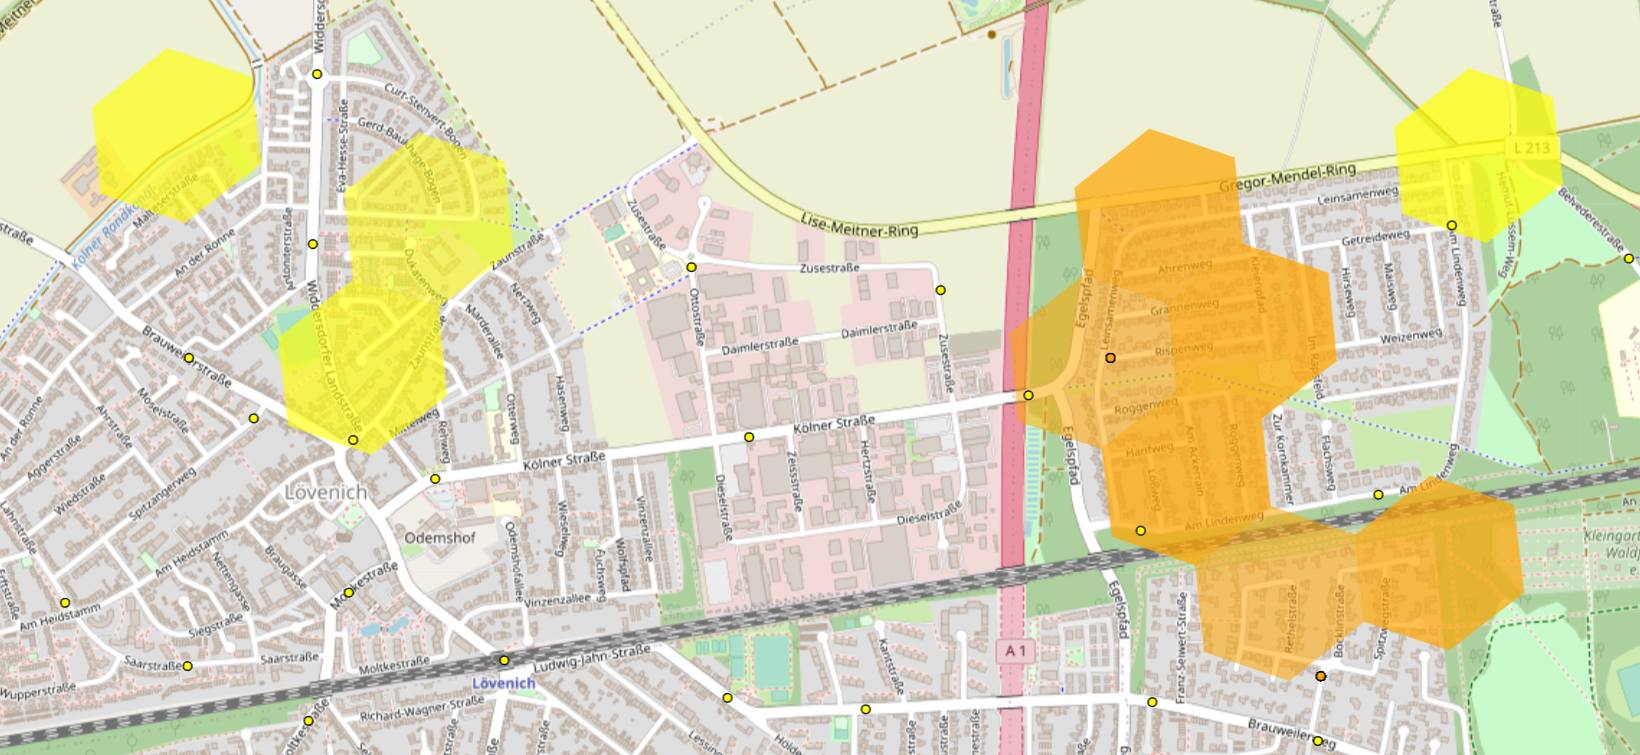
\includegraphics[width=\textwidth]{Figures/results/problematic_hexagons/example_2.png}
     \end{subfigure}
     \hfill
     \begin{subfigure}[b]{0.45\textwidth}
         \centering
         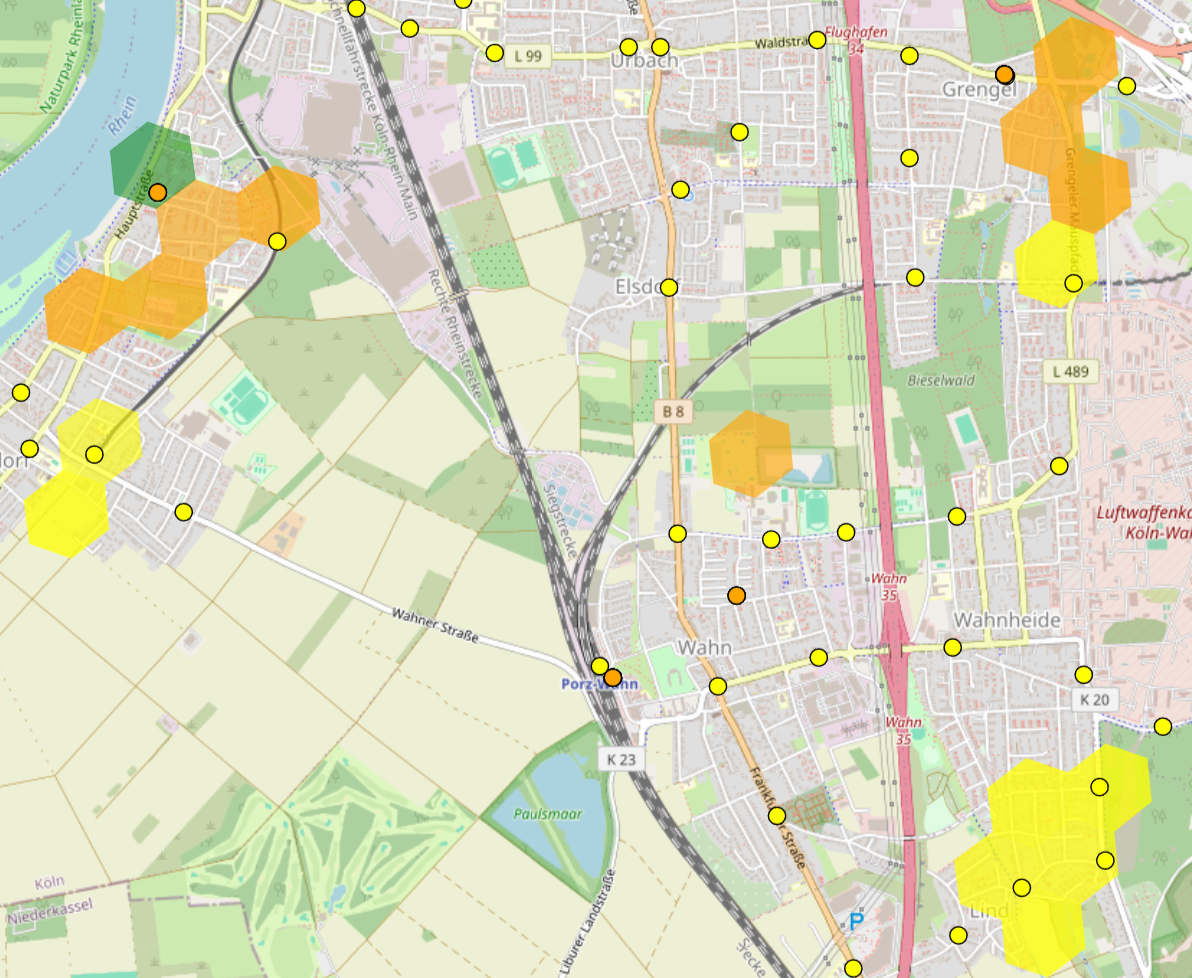
\includegraphics[width=\textwidth]{Figures/results/problematic_hexagons/example_3.png}
     \end{subfigure}
     \hfill
     \begin{subfigure}[b]{0.45\textwidth}
         \centering
         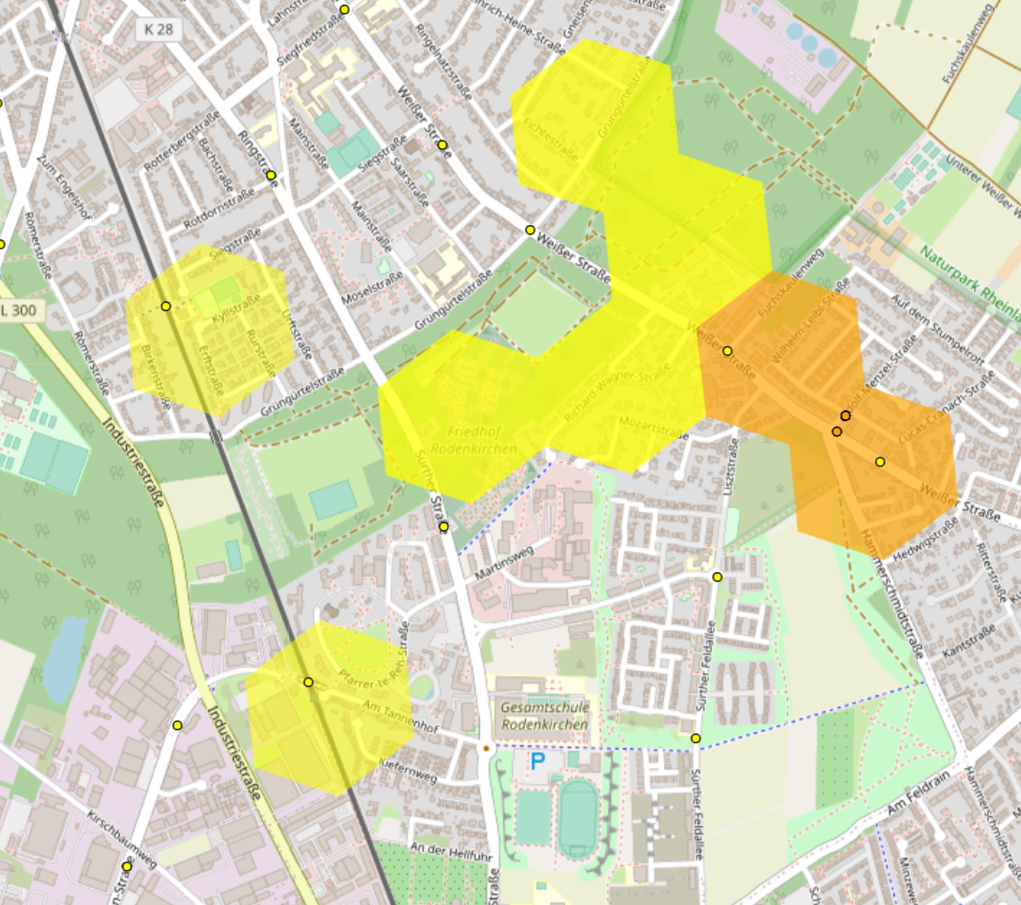
\includegraphics[width=\textwidth]{Figures/results/problematic_hexagons/example_4.png}
     \end{subfigure}
     \caption{Examples of fixable hexagons}
        \label{fig:fixable_hexagons_examples}
\end{figure}

Public Transport stops are visualized as yellow circles, while bicycles are visualized as orange circles.
We see that hexagons that are fixed in the bicycle sharing scenario are always close to orange cycles.
Similarly, hexagons that are fixed in the public transport scenario are always close to public transport stops.
However, the proximity to bicycles seems to have a larger influence than the proximity to public transport stops.


Figure \ref{fig:only_unfixable_hexagons} shows all hexagons that are not 15-minute hexagons by any sustainable mode of transport.
Figure \ref{fig:unfixable_with_bicycles} and \ref{fig:unfixable_with_stops} show the same map, but with additional bicycle locations and public transport stop locations, respectively.

\begin{figure}
     \centering
     \begin{subfigure}[b]{0.30\textwidth}
         \centering
         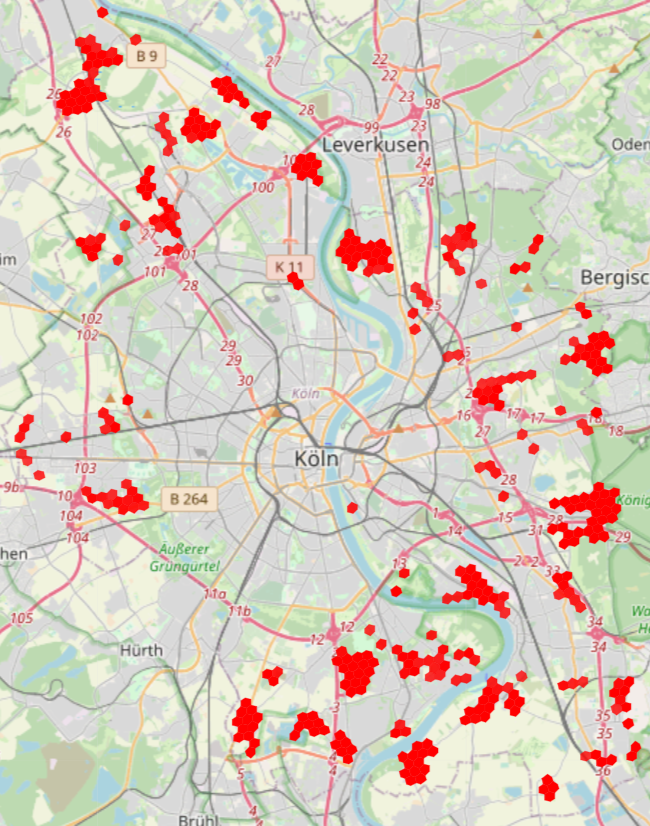
\includegraphics[width=\textwidth]{Figures/results/problematic_hexagons/unfixable.png}
         \caption{Only Unfixable hexagons}
         \label{fig:only_unfixable_hexagons}
     \end{subfigure}
     \hfill
     \begin{subfigure}[b]{0.30\textwidth}
         \centering
         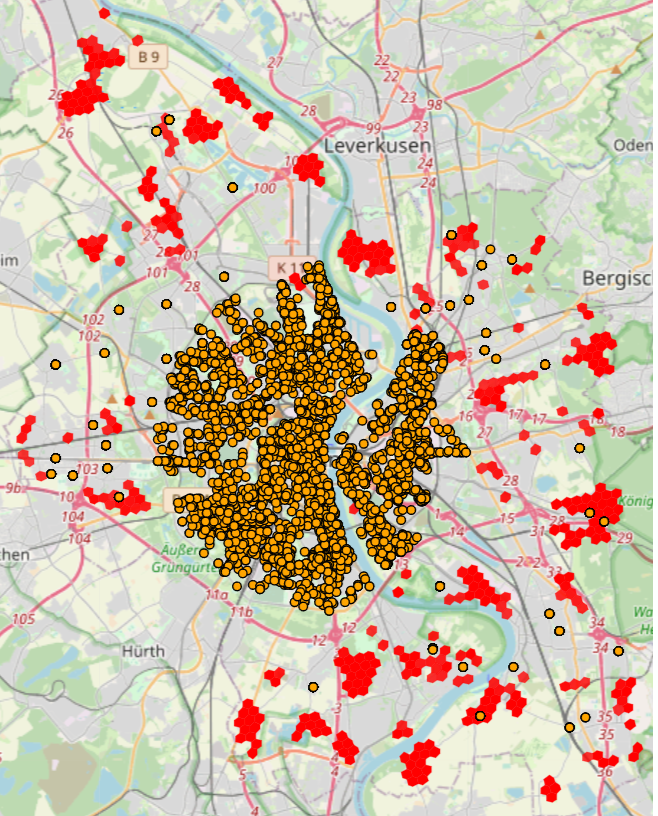
\includegraphics[width=\textwidth]{Figures/results/problematic_hexagons/unfixable_with_bicycles.png}
         \caption{With all bicycle locations}
         \label{fig:unfixable_with_bicycles}
     \end{subfigure}
     \hfill
     \begin{subfigure}[b]{0.30\textwidth}
         \centering
         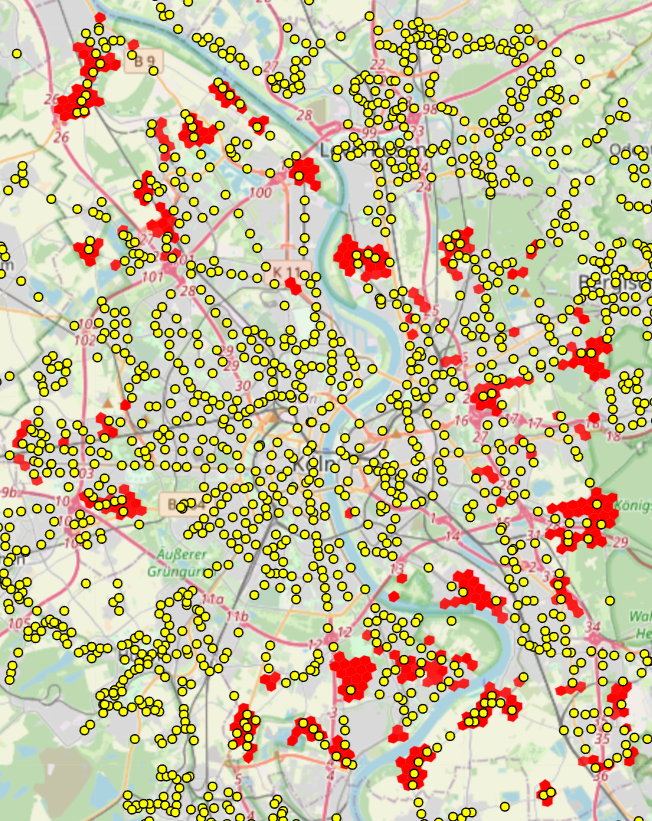
\includegraphics[width=\textwidth]{Figures/results/problematic_hexagons/unfixable_with_stops.png}
         \caption{With public transport stops}
         \label{fig:unfixable_with_stops}
     \end{subfigure}
     \hfill
     \caption{Unfixable hexagons}
     \label{fig:unfixable_hexagons}
\end{figure}

We can observe that the unfixable hexagons mostly don't contain any bicycles and have a larger distance to the next bicycle.
The same cannot be said for public transport stops.
Often public transport stops are directly inside the unfixable hexagons.


Figure \ref{fig:combined_hexagons} shows all hexagons that only become 15-minute city hexagons in the combined scenario, which means when both public transport and bicycle sharing can be used at the same time.
As already seen in Table \ref{table:hexagons_with_walking_time_above_15_minutes} this only concerns less than 2\% of all hexagons that are not already 15-minute city hexagons through walking alone.
More than half of those (7 out of 10) are located in the district of Weiß.


\begin{figure}
  \begin{center}
    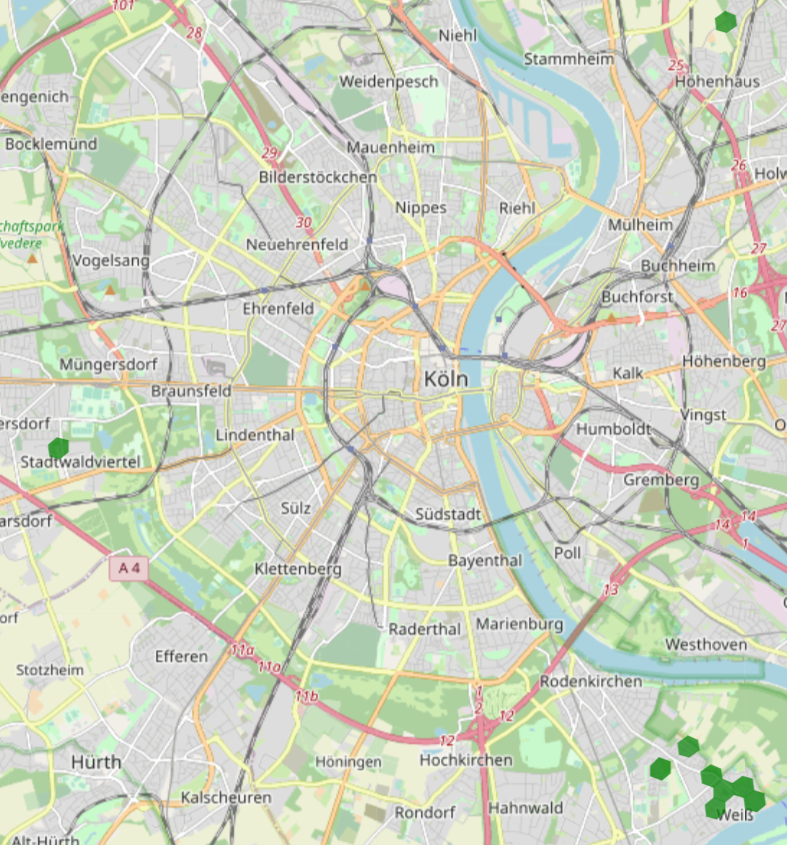
\includegraphics[width=0.50\textwidth]{Figures/results/problematic_hexagons/combined_hexagons}
  \end{center}
  \caption{Hexagons fixable by combined mode}
  \label{fig:combined_hexagons}
\end{figure}
